% Options for packages loaded elsewhere
\PassOptionsToPackage{unicode}{hyperref}
\PassOptionsToPackage{hyphens}{url}
%
\documentclass[
  8pt,
  ignorenonframetext,
]{beamer}
\usepackage{pgfpages}
\setbeamertemplate{caption}[numbered]
\setbeamertemplate{caption label separator}{: }
\setbeamercolor{caption name}{fg=normal text.fg}
\beamertemplatenavigationsymbolsempty
% Prevent slide breaks in the middle of a paragraph
\widowpenalties 1 10000
\raggedbottom
\setbeamertemplate{part page}{
  \centering
  \begin{beamercolorbox}[sep=16pt,center]{part title}
    \usebeamerfont{part title}\insertpart\par
  \end{beamercolorbox}
}
\setbeamertemplate{section page}{
  \centering
  \begin{beamercolorbox}[sep=12pt,center]{part title}
    \usebeamerfont{section title}\insertsection\par
  \end{beamercolorbox}
}
\setbeamertemplate{subsection page}{
  \centering
  \begin{beamercolorbox}[sep=8pt,center]{part title}
    \usebeamerfont{subsection title}\insertsubsection\par
  \end{beamercolorbox}
}
\AtBeginPart{
  \frame{\partpage}
}
\AtBeginSection{
  \ifbibliography
  \else
    \frame{\sectionpage}
  \fi
}
\AtBeginSubsection{
  \frame{\subsectionpage}
}
\usepackage{amsmath,amssymb}
\usepackage{lmodern}
\usepackage{iftex}
\ifPDFTeX
  \usepackage[T1]{fontenc}
  \usepackage[utf8]{inputenc}
  \usepackage{textcomp} % provide euro and other symbols
\else % if luatex or xetex
  \usepackage{unicode-math}
  \defaultfontfeatures{Scale=MatchLowercase}
  \defaultfontfeatures[\rmfamily]{Ligatures=TeX,Scale=1}
\fi
% Use upquote if available, for straight quotes in verbatim environments
\IfFileExists{upquote.sty}{\usepackage{upquote}}{}
\IfFileExists{microtype.sty}{% use microtype if available
  \usepackage[]{microtype}
  \UseMicrotypeSet[protrusion]{basicmath} % disable protrusion for tt fonts
}{}
\makeatletter
\@ifundefined{KOMAClassName}{% if non-KOMA class
  \IfFileExists{parskip.sty}{%
    \usepackage{parskip}
  }{% else
    \setlength{\parindent}{0pt}
    \setlength{\parskip}{6pt plus 2pt minus 1pt}}
}{% if KOMA class
  \KOMAoptions{parskip=half}}
\makeatother
\usepackage{xcolor}
\newif\ifbibliography
\usepackage{color}
\usepackage{fancyvrb}
\newcommand{\VerbBar}{|}
\newcommand{\VERB}{\Verb[commandchars=\\\{\}]}
\DefineVerbatimEnvironment{Highlighting}{Verbatim}{commandchars=\\\{\}}
% Add ',fontsize=\small' for more characters per line
\usepackage{framed}
\definecolor{shadecolor}{RGB}{248,248,248}
\newenvironment{Shaded}{\begin{snugshade}}{\end{snugshade}}
\newcommand{\AlertTok}[1]{\textcolor[rgb]{0.94,0.16,0.16}{#1}}
\newcommand{\AnnotationTok}[1]{\textcolor[rgb]{0.56,0.35,0.01}{\textbf{\textit{#1}}}}
\newcommand{\AttributeTok}[1]{\textcolor[rgb]{0.77,0.63,0.00}{#1}}
\newcommand{\BaseNTok}[1]{\textcolor[rgb]{0.00,0.00,0.81}{#1}}
\newcommand{\BuiltInTok}[1]{#1}
\newcommand{\CharTok}[1]{\textcolor[rgb]{0.31,0.60,0.02}{#1}}
\newcommand{\CommentTok}[1]{\textcolor[rgb]{0.56,0.35,0.01}{\textit{#1}}}
\newcommand{\CommentVarTok}[1]{\textcolor[rgb]{0.56,0.35,0.01}{\textbf{\textit{#1}}}}
\newcommand{\ConstantTok}[1]{\textcolor[rgb]{0.00,0.00,0.00}{#1}}
\newcommand{\ControlFlowTok}[1]{\textcolor[rgb]{0.13,0.29,0.53}{\textbf{#1}}}
\newcommand{\DataTypeTok}[1]{\textcolor[rgb]{0.13,0.29,0.53}{#1}}
\newcommand{\DecValTok}[1]{\textcolor[rgb]{0.00,0.00,0.81}{#1}}
\newcommand{\DocumentationTok}[1]{\textcolor[rgb]{0.56,0.35,0.01}{\textbf{\textit{#1}}}}
\newcommand{\ErrorTok}[1]{\textcolor[rgb]{0.64,0.00,0.00}{\textbf{#1}}}
\newcommand{\ExtensionTok}[1]{#1}
\newcommand{\FloatTok}[1]{\textcolor[rgb]{0.00,0.00,0.81}{#1}}
\newcommand{\FunctionTok}[1]{\textcolor[rgb]{0.00,0.00,0.00}{#1}}
\newcommand{\ImportTok}[1]{#1}
\newcommand{\InformationTok}[1]{\textcolor[rgb]{0.56,0.35,0.01}{\textbf{\textit{#1}}}}
\newcommand{\KeywordTok}[1]{\textcolor[rgb]{0.13,0.29,0.53}{\textbf{#1}}}
\newcommand{\NormalTok}[1]{#1}
\newcommand{\OperatorTok}[1]{\textcolor[rgb]{0.81,0.36,0.00}{\textbf{#1}}}
\newcommand{\OtherTok}[1]{\textcolor[rgb]{0.56,0.35,0.01}{#1}}
\newcommand{\PreprocessorTok}[1]{\textcolor[rgb]{0.56,0.35,0.01}{\textit{#1}}}
\newcommand{\RegionMarkerTok}[1]{#1}
\newcommand{\SpecialCharTok}[1]{\textcolor[rgb]{0.00,0.00,0.00}{#1}}
\newcommand{\SpecialStringTok}[1]{\textcolor[rgb]{0.31,0.60,0.02}{#1}}
\newcommand{\StringTok}[1]{\textcolor[rgb]{0.31,0.60,0.02}{#1}}
\newcommand{\VariableTok}[1]{\textcolor[rgb]{0.00,0.00,0.00}{#1}}
\newcommand{\VerbatimStringTok}[1]{\textcolor[rgb]{0.31,0.60,0.02}{#1}}
\newcommand{\WarningTok}[1]{\textcolor[rgb]{0.56,0.35,0.01}{\textbf{\textit{#1}}}}
\usepackage{longtable,booktabs,array}
\usepackage{calc} % for calculating minipage widths
\usepackage{caption}
% Make caption package work with longtable
\makeatletter
\def\fnum@table{\tablename~\thetable}
\makeatother
\setlength{\emergencystretch}{3em} % prevent overfull lines
\providecommand{\tightlist}{%
  \setlength{\itemsep}{0pt}\setlength{\parskip}{0pt}}
\setcounter{secnumdepth}{-\maxdimen} % remove section numbering
\newlength{\cslhangindent}
\setlength{\cslhangindent}{1.5em}
\newlength{\csllabelwidth}
\setlength{\csllabelwidth}{3em}
\newlength{\cslentryspacingunit} % times entry-spacing
\setlength{\cslentryspacingunit}{\parskip}
\newenvironment{CSLReferences}[2] % #1 hanging-ident, #2 entry spacing
 {% don't indent paragraphs
  \setlength{\parindent}{0pt}
  % turn on hanging indent if param 1 is 1
  \ifodd #1
  \let\oldpar\par
  \def\par{\hangindent=\cslhangindent\oldpar}
  \fi
  % set entry spacing
  \setlength{\parskip}{#2\cslentryspacingunit}
 }%
 {}
\usepackage{calc}
\newcommand{\CSLBlock}[1]{#1\hfill\break}
\newcommand{\CSLLeftMargin}[1]{\parbox[t]{\csllabelwidth}{#1}}
\newcommand{\CSLRightInline}[1]{\parbox[t]{\linewidth - \csllabelwidth}{#1}\break}
\newcommand{\CSLIndent}[1]{\hspace{\cslhangindent}#1}
% type setting
% ------------------------------------------------------------------------------
\usepackage[german]{babel}     

% fonts
% ------------------------------------------------------------------------------
\usefonttheme{professionalfonts}

% slide title and horizontal line
% ------------------------------------------------------------------------------
\setbeamertemplate{frametitle}{%
    \vskip-30pt \color{black}\large%
    \begin{minipage}[b][23pt]{120mm}%
    \flushleft\insertframetitle%
    \end{minipage}%
}

\setbeamertemplate{headline}										
{
\vskip10pt\hfill\hspace{3.5mm} 										 
\vskip15pt\color{black}\rule{\textwidth}{0.4pt} 					 
}

% slide number
% ---------------------------------------------------------------
\setbeamertemplate{navigation symbols}{}
\setbeamertemplate{footline}
{
\vskip5pt
\vskip2pt
\makebox[123mm]{\hspace{7.5mm}
\hfill Multivariate Datenanalyse $\vert$ 
\copyright $ $ 2023 Dirk Ostwald CC BY-SA 4.0 $\vert$ 
Folie \insertframenumber}
\vskip4pt
}

% block color scheme
% ------------------------------------------------------------------------------
% colors
\definecolor{white}{RGB}{255,255,255}
\definecolor{grey}{RGB}{235,235,235}
\definecolor{lightgrey}{RGB}{245,245,245}
\definecolor{LightBlue}{RGB}{220,220,255}
\definecolor{darkblue}{RGB}{51, 51, 153}

% definitions and theorems
\setbeamercolor{block title}{fg = black, bg = grey}
\setbeamercolor{block body}{fg = black, bg = lightgrey}

% general line spacing 
% ------------------------------------------------------------------------------
\linespread{1.3}

% local line spacing
% ------------------------------------------------------------------------------
\usepackage{setspace}

% colors
% -----------------------------------------------------------------------------
\usepackage{color}

% justified text
% ------------------------------------------------------------------------------
\usepackage{tabularx}
\usepackage{ragged2e}
\usepackage{etoolbox}
\apptocmd{\frame}{}{\justifying}{}

% bullet point lists
% -----------------------------------------------------------------------------
\setbeamertemplate{itemize item}[circle]
\setbeamertemplate{itemize subitem}[circle]
\setbeamertemplate{itemize subsubitem}[circle]
\setbeamercolor{itemize item}{fg = black}
\setbeamercolor{itemize subitem}{fg = black}
\setbeamercolor{itemize subsubitem}{fg = black}
\setbeamercolor{enumerate item}{fg = black}
\setbeamercolor{enumerate subitem}{fg = black}
\setbeamercolor{enumerate subsubitem}{fg = black}
\setbeamerfont{itemize/enumerate body}{}
\setbeamerfont{itemize/enumerate subbody}{size = \normalsize}
\setbeamerfont{itemize/enumerate subsubbody}{size = \normalsize}

% color links
% ------------------------------------------------------------------------------
\usepackage{hyperref}
\definecolor{urls}{RGB}{204,0,0}
\hypersetup{colorlinks, citecolor = darkblue, urlcolor = urls}


% additional math commands
% ------------------------------------------------------------------------------
\usepackage{bm}                                          
\usepackage{mathtools}                         
\newcommand{\niton}{\not\owns}
\newcommand{\ups}{\upsilon}
\DeclareMathOperator*{\argmax}{arg\,max}
\DeclareMathOperator*{\argmin}{arg\,min}

% text highlighting
% ------------------------------------------------------------------------------
\usepackage{soul}
\makeatletter
\let\HL\hl
\renewcommand\hl{%
  \let\set@color\beamerorig@set@color
  \let\reset@color\beamerorig@reset@color
  \HL}
\makeatother

% equation highlighting
% -----------------------------------------------------------------------------
\newcommand{\highlight}[2][yellow]{\mathchoice%
  {\colorbox{#1}{$\displaystyle#2$}}%
  {\colorbox{#1}{$\textstyle#2$}}%
  {\colorbox{#1}{$\scriptstyle#2$}}%
  {\colorbox{#1}{$\scriptscriptstyle#2$}}}%
  
\ifLuaTeX
  \usepackage{selnolig}  % disable illegal ligatures
\fi
\IfFileExists{bookmark.sty}{\usepackage{bookmark}}{\usepackage{hyperref}}
\IfFileExists{xurl.sty}{\usepackage{xurl}}{} % add URL line breaks if available
\urlstyle{same} % disable monospaced font for URLs
\hypersetup{
  hidelinks,
  pdfcreator={LaTeX via pandoc}}

\author{}
\date{\vspace{-2.5em}}

\begin{document}

\begin{frame}[plain]{}
\protect\hypertarget{section}{}
\center

\begin{center}
\includegraphics[width=0.2\linewidth]{7_Abbildungen/mvda_7_otto} \end{center}

\vspace{2mm}

\Huge

Multivariate Datenanalyse \vspace{6mm}

\Large

MSc Psychologie WiSe 2022/23

\vspace{6mm}
\large

Prof.~Dr.~Dirk Ostwald
\end{frame}

\begin{frame}[plain]{}
\protect\hypertarget{section-1}{}
\vfill
\center
\huge

\textcolor{black}{(7) Kanonische Korrelationsanalyse} \vfill
\end{frame}

\begin{frame}{}
\protect\hypertarget{section-2}{}
\vspace{2mm}

\textcolor{darkblue}{Modul A1/A3 Forschungsmethoden: Multivariate Verfahren | Themen}
\vspace{2mm}

\center
\footnotesize
\renewcommand{\arraystretch}{1.1}
\begin{tabular}{lll}
Datum        & Einheit                          & Thema                                       \\\hline
14.10.2022   & Grundlagen                       & (1) Einführung                              \\
21.10.2022   & Grundlagen                       & (2) Vektoren                                \\
28.10.2022   & Grundlagen                       & (3) Matrizen                                \\
04.11.2022   & Grundlagen                       & (4) Eigenanalyse                            \\
11.11.2022   & Grundlagen                       & (5) Multivariate Wahrscheinlichkeitstheorie \\
18.11.2022   & Grundlagen                       & (6) Multivariate Normalverteilungen         \\
25.11.2022   & Frequentistische Inferenz        & (7) Kanonische Korrelationsanalyse          \\
02.12.2022   & Frequentistische Inferenz        & (8) T$^2$-Tests                             \\
09.12.2022   & Frequentistische Inferenz        & (9) Einfaktorielle MANOVA                   \\
16.12.2022   & Latente Variablenmodelle         & (10) Hauptkomponentenanalyse                \\
             & \textcolor{gray}{Weihnachtspause}                                              \\
13.01.2023   & Latente Variablenmodelle         & (12) Lineare Normalverteilungsmodelle       \\
20.01.2023   & Latente Variablenmodelle         & (13) Konfirmatorische Faktorenanalyse       \\
27.01.2023   & Latente Variablenmodelle         & (14) Exploratorische Faktorenanalyse        \\ 
\end{tabular}
\end{frame}

\begin{frame}{Frequentistische Inferenz}
\protect\hypertarget{frequentistische-inferenz}{}
\textcolor{darkblue}{Datenanalyseszenarien} \vspace{2mm}

\small
\renewcommand{\arraystretch}{2}
\begin{tabular}{lll}
UV
& AV
& Datenanalysemethoden
\\\hline
Univariat
& Univariat
& Korrelation, Einfache Regression,T-Tests
\\
Multivariat
& Univariat
& Multiple Korrelation, Multiple Regression, Allgemeines Lineares Modell
\\
Univariat
& Multivariat
& T$^2$-Tests, Einfaktorielle MANOVA
\\
Multivariat
& Multivariat
& Kanonische Korrelation, Multivariates Allgemeines Lineares Modell
\end{tabular}
\end{frame}

\begin{frame}{Frequentistische Inferenz}
\protect\hypertarget{frequentistische-inferenz-1}{}
\textcolor{darkblue}{Datenanalyseszenarien} \vspace{4mm}

\small
\begin{minipage}{0.5\linewidth}
\center
\begin{tabular}{c|c}
UV         & AV          \\
$x_1$      & $y_1$       \\\hline
$x_{11}$   & $y_{11}$    \\
$x_{12}$   & $y_{12}$    \\
$x_{13}$   & $y_{13}$    \\
$\vdots$   & $\vdots$    \\
$\vdots$   & $\vdots$    \\
$\vdots$   & $\vdots$    \\
$x_{1n}$   & $y_{1n}$    \\
\end{tabular}
\vspace{2mm}

Korrelation

Einfache Regression

T-Tests
\end{minipage}
\begin{minipage}{0.5\linewidth}
\center
\begin{tabular}{ccc|c}
          & UV        &          & AV          \\
$x_1$     & $\cdots$  & $x_m$    & $y_1$       \\\hline
$x_{11}$  & $\cdots$  & $x_{m1}$ & $y_{11}$    \\
$x_{12}$  & $\cdots$  & $x_{m2}$ & $y_{12}$    \\
$x_{13}$  & $\cdots$  & $x_{m3}$ & $y_{13}$    \\
$\vdots$  & $\vdots$  & $\vdots$ & $\vdots$    \\
$\vdots$  & $\vdots$  & $\vdots$ & $\vdots$    \\
$\vdots$  & $\vdots$  & $\vdots$ & $\vdots$    \\
$x_{1n}$  & $\cdots$  & $x_{mn}$ & $y_{1n}$    \\
\end{tabular}
\vspace{2mm}

Multiple Korrelation

Multiple Regression

Allgemeines Lineares Modell

\end{minipage}
\end{frame}

\begin{frame}{Frequentistische Inferenz}
\protect\hypertarget{frequentistische-inferenz-2}{}
\textcolor{darkblue}{Datenanalyseszenarien} \vspace{4mm}

\small
\begin{minipage}{0.4\linewidth}
\center
\begin{tabular}{c|ccc}
UV        &          & AV        &             \\
$x_1$     & $y_1$    & $\cdots$  & $y_m$       \\\hline
$x_{11}$  & $y_{12}$ & $\cdots$  & $y_{m1}$    \\
$x_{12}$  & $y_{13}$ & $\cdots$  & $y_{m2}$    \\
$x_{13}$  & $y_{14}$ & $\cdots$  & $y_{m3}$    \\
$\vdots$  & $\vdots$ & $\vdots$  & $\vdots$    \\
$\vdots$  & $\vdots$ & $\vdots$  & $\vdots$    \\
$\vdots$  & $\vdots$ & $\vdots$  & $\vdots$    \\
$x_{1n}$  & $y_{1n}$ & $\cdots$  & $y_{mn}$    \\
\end{tabular}
\vspace{2mm}

T$^2$-Tests

Einfaktorielle MANOVA

\end{minipage}\hspace{2mm}
\begin{minipage}{0.6\linewidth}
\center
\begin{tabular}{ccc|ccc}
          & UV        &             &            & AV        &             \\
$x_1$     & $\cdots$  & $x_{m_x}$   & $y_1$      & $\cdots$  & $y_{m_y}$   \\\hline
$x_{11}$  & $\cdots$  & $x_{m_x1}$  & $y_{11}$   & $\cdots$  & $y_{m_y1}$  \\
$x_{12}$  & $\cdots$  & $x_{m_x2}$  & $y_{12}$   & $\cdots$  & $y_{m_y2}$  \\
$x_{13}$  & $\cdots$  & $x_{m_x3}$  & $y_{13}$   & $\cdots$  & $y_{m_y3}$  \\
$\vdots$  & $\vdots$  & $\vdots$    & $\vdots$   & $\vdots$  & $\vdots$    \\
$\vdots$  & $\vdots$  & $\vdots$    & $\vdots$   & $\vdots$  & $\vdots$    \\
$\vdots$  & $\vdots$  & $\vdots$    & $\vdots$   & $\vdots$  & $\vdots$    \\
$x_{1n}$  & $\cdots$  & $x_{m_xn}$  & $y_{1n}$   & $\cdots$  & $y_{m_yn}$  \\
\end{tabular}
\vspace{2mm}

\textbf{Kanonische Korrelationsanalyse}

Multivariates Allgemeines Lineares Modell
\end{minipage}
\end{frame}

\begin{frame}{}
\protect\hypertarget{section-3}{}
\setstretch{2.5}
\vfill
\large

Korrelation

Algebraische Grundlagen

Wahrscheinlichkeitstheoretische Grundlagen

Modellformulierung

Modellschätzung

Selbstkontrollfragen \vfill
\end{frame}

\begin{frame}{}
\protect\hypertarget{section-4}{}
\setstretch{2.5}
\vfill
\large

\textbf{Korrelation}

Algebraische Grundlagen

Wahrscheinlichkeitstheoretische Grundlagen

Modellformulierung

Modellschätzung

Selbstkontrollfragen \vfill
\end{frame}

\begin{frame}{Korrelation}
\protect\hypertarget{korrelation}{}
\large

Anwendungsszenario \vspace{2mm}

\begin{center}
\includegraphics[width=0.8\linewidth]{7_Abbildungen/mvda_7_beispielszenario_korrelation} \end{center}
\end{frame}

\begin{frame}{Grundlagen}
\protect\hypertarget{grundlagen}{}
Beispieldatensatz

\center
\footnotesize

\(i = 1,...,20\) Patient:innen, \(y_i\) Symptomreduktion bei Patient:in
\(i\), \(x_i\) Anzahl Therapiestunden von Patient:in \(i\)

\setstretch{1}

\setstretch{1}

\begin{longtable}[]{@{}rr@{}}
\toprule()
x\_i & y\_i \\
\midrule()
\endhead
27.9 & 35.5 \\
15.3 & 25.0 \\
17.4 & 19.7 \\
21.5 & 28.8 \\
28.2 & 29.4 \\
14.0 & 17.2 \\
28.0 & 32.9 \\
28.9 & 28.3 \\
23.2 & 25.8 \\
22.6 & 31.3 \\
11.2 & 14.4 \\
14.1 & 18.4 \\
13.5 & 19.1 \\
23.7 & 28.0 \\
17.7 & 20.3 \\
25.4 & 34.8 \\
20.0 & 27.6 \\
24.4 & 31.9 \\
29.8 & 32.2 \\
17.6 & 24.6 \\
\bottomrule()
\end{longtable}
\end{frame}

\begin{frame}{Korrelation}
\protect\hypertarget{korrelation-1}{}
Beispieldatensatz

\begin{center}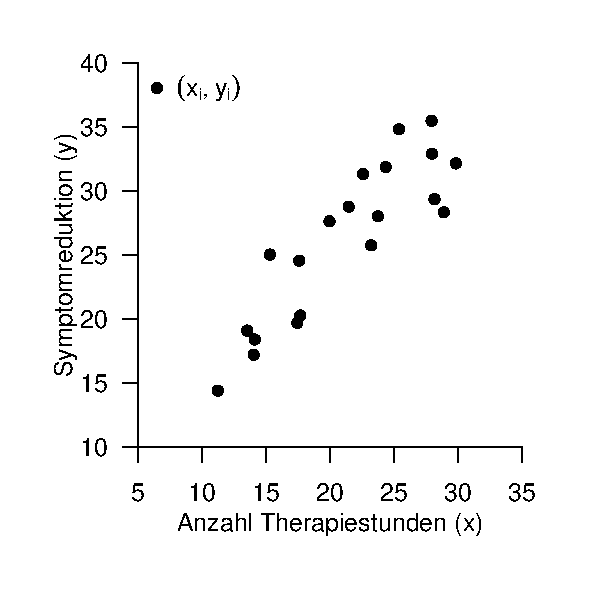
\includegraphics[width=0.55\linewidth]{7_Abbildungen/mvda_7_beispieldatensatz_korrelation} \end{center}

\center

\textcolor{darkblue}{Wie stark hängen Anzahl Therapiestunden und Symptomreduktion zusammen?}
\end{frame}

\begin{frame}{Korrelation}
\protect\hypertarget{korrelation-2}{}
\small
\begin{definition}[Korrelation]
\justifying
Die \textit{Korrelation} zweier Zufallsvariablen $\xi$ und $\ups$ ist definiert als
\begin{equation}
\rho(\xi,\ups) := \frac{\mathbb{C}(\xi,\ups)}{\sqrt{\mathbb{V}(\xi)}\sqrt{\mathbb{V}(\ups)}}
\end{equation}
wobei $\mathbb{C}(\xi,\ups)$ die Kovarianz von $\xi$ und $\ups$ und $\mathbb{V}(\xi)$ und
$\mathbb{V}(\ups)$ die Varianzen von $\xi$ und $\ups$ bezeichnen.
\end{definition}

\small

Für eine Einführung zur Korrelation siehe die entsprechenden BSc
Lehreinheiten

\href{https://youtu.be/613-3a1Pyyg}{\textcolor{darkblue}{$\bullet$ Erwartungswert, Varianz, Kovarianz}}

\href{https://youtu.be/zfI6LoX8bc4}{\textcolor{darkblue}{$\bullet$ Korrelation}}

\footnotesize

Bemerkungen

\begin{itemize}
\tightlist
\item
  \(\rho(\xi,\ups)\) wird auch \textit{Korrelationskoeffizient} von
  \(\xi\) und \(\ups\) genannt.
\item
  Wir haben bereits gesehen, dass \(-1 \le \rho(\xi,\ups) \le 1\) gilt.
\item
  Wenn \(\rho(\xi,\ups) = 0\) ist, werden \(\xi\) und \(\ups\)
  \textit{unkorreliert} genannt.
\item
  Aus der Unabhängigkeit von \(\xi\) und \(\ups\) folgt
  \(\rho(\xi,\ups) = 0\).
\item
  Aus \(\rho(\xi,\ups) = 0\) folgt die Unabhängigkeit von \(\xi\) und
  \(\ups\) im Allgemeinen nicht.
\end{itemize}
\end{frame}

\begin{frame}{Korrelation}
\protect\hypertarget{korrelation-3}{}
\footnotesize
\begin{definition}[Stichprobenkorrelation]
\justifying
$(x_1,y_1),...,(x_n,y_n)$ seien Realisierungen von zweidimensionalen Zufallsvektoren
$(\xi_1,\ups_1), ..., (\xi_n,\ups_n)$. Weiterhin seien:
\begin{itemize}
\item Die Stichprobenmittel der $x_i$ und $y_i$ definiert als
\begin{equation}
\bar{x} := \frac{1}{n}\sum_{i=1}^n x_i
\mbox{ und }
\bar{y} := \frac{1}{n}\sum_{i=1}^n y_i.
\end{equation}
\item Die Stichprobenstandardabweichungen $x_i$ und $y_i$ definiert als
\begin{equation}
s_x := \sqrt{\frac{1}{n-1}(x_i - \bar{x})^2}
\mbox{ und }
s_y := \sqrt{\frac{1}{n-1}(y_i - \bar{y})^2}.
\end{equation}
\item Die Stichprobenkovarianz der $(x_1,y_1),...,(x_n,y_n)$ definiert als
\begin{equation}
c_{xy} := \frac{1}{n-1}\sum_{i=1}^n (x_i - \bar{x})(y_i - \bar{y}).
\end{equation}
\end{itemize}
Dann ist die \textit{Stichprobenkorrelation} der $(x_1,y_1),...,(x_n,y_n)$ definiert als
\begin{equation}
r_{xy} := \frac{c_{xy}}{s_xs_y}
\end{equation}
und  wird auch \textit{Stichprobenkorrelationskoeffizient} genannt.
\end{definition}
\end{frame}

\begin{frame}[fragile]{Korrelation}
\protect\hypertarget{korrelation-4}{}
Beispiel \vspace{2mm} \tiny \setstretch{1.2}

\begin{Shaded}
\begin{Highlighting}[]
\CommentTok{\# Laden des Beispieldatensatzes}
\NormalTok{fname }\OtherTok{=} \FunctionTok{file.path}\NormalTok{(}\FunctionTok{getwd}\NormalTok{(), }\StringTok{"7\_Kanonische\_Korrelationsanalyse.csv"}\NormalTok{)                }\CommentTok{\# Dateipfad}
\NormalTok{D     }\OtherTok{=} \FunctionTok{read.table}\NormalTok{(fname, }\AttributeTok{sep =} \StringTok{","}\NormalTok{, }\AttributeTok{header =} \ConstantTok{TRUE}\NormalTok{)                              }\CommentTok{\# Laden als Dataframe}
\NormalTok{x\_i   }\OtherTok{=}\NormalTok{ D}\SpecialCharTok{$}\NormalTok{x\_1i                                                                    }\CommentTok{\# x\_i Werte}
\NormalTok{y\_i   }\OtherTok{=}\NormalTok{ D}\SpecialCharTok{$}\NormalTok{y\_1i                                                                    }\CommentTok{\# y\_i Werte}
\NormalTok{n     }\OtherTok{=} \FunctionTok{length}\NormalTok{(x\_i)                                                              }\CommentTok{\# n}

\CommentTok{\# "Manuelle" Berechnung der Stichprobenkorrelation}
\NormalTok{x\_bar }\OtherTok{=}\NormalTok{ (}\DecValTok{1}\SpecialCharTok{/}\NormalTok{n)}\SpecialCharTok{*}\FunctionTok{sum}\NormalTok{(x\_i)                                                           }\CommentTok{\# \textbackslash{}bar\{x\}}
\NormalTok{y\_bar }\OtherTok{=}\NormalTok{ (}\DecValTok{1}\SpecialCharTok{/}\NormalTok{n)}\SpecialCharTok{*}\FunctionTok{sum}\NormalTok{(y\_i)                                                           }\CommentTok{\# \textbackslash{}bar\{y\}}
\NormalTok{s\_x   }\OtherTok{=} \FunctionTok{sqrt}\NormalTok{(}\DecValTok{1}\SpecialCharTok{/}\NormalTok{(n}\DecValTok{{-}1}\NormalTok{)}\SpecialCharTok{*}\FunctionTok{sum}\NormalTok{((x\_i }\SpecialCharTok{{-}}\NormalTok{ x\_bar)}\SpecialCharTok{\^{}}\DecValTok{2}\NormalTok{))                                       }\CommentTok{\# s\_x}
\NormalTok{s\_y   }\OtherTok{=} \FunctionTok{sqrt}\NormalTok{(}\DecValTok{1}\SpecialCharTok{/}\NormalTok{(n}\DecValTok{{-}1}\NormalTok{)}\SpecialCharTok{*}\FunctionTok{sum}\NormalTok{((y\_i }\SpecialCharTok{{-}}\NormalTok{ y\_bar)}\SpecialCharTok{\^{}}\DecValTok{2}\NormalTok{))                                       }\CommentTok{\# s\_y}
\NormalTok{c\_xy  }\OtherTok{=} \DecValTok{1}\SpecialCharTok{/}\NormalTok{(n}\DecValTok{{-}1}\NormalTok{) }\SpecialCharTok{*} \FunctionTok{sum}\NormalTok{((x\_i }\SpecialCharTok{{-}}\NormalTok{ x\_bar) }\SpecialCharTok{*}\NormalTok{ (y\_i }\SpecialCharTok{{-}}\NormalTok{ y\_bar))                             }\CommentTok{\# c\_\{xy\}}
\NormalTok{r\_xy  }\OtherTok{=}\NormalTok{ c\_xy}\SpecialCharTok{/}\NormalTok{(s\_x }\SpecialCharTok{*}\NormalTok{ s\_y)                                                         }\CommentTok{\# r\_\{xy\}}
\FunctionTok{print}\NormalTok{(r\_xy)                                                                      }\CommentTok{\# Ausgabe}
\end{Highlighting}
\end{Shaded}

\begin{verbatim}
> [1] 0.883
\end{verbatim}

\begin{Shaded}
\begin{Highlighting}[]
\CommentTok{\# Automatische Berechnung mit cor()}
\NormalTok{r\_xy  }\OtherTok{=} \FunctionTok{cor}\NormalTok{(x\_i,y\_i)                                                             }\CommentTok{\# r\_\{xy\}}
\FunctionTok{print}\NormalTok{(r\_xy)                                                                      }\CommentTok{\# Ausgabe}
\end{Highlighting}
\end{Shaded}

\begin{verbatim}
> [1] 0.883
\end{verbatim}

\center
\small

\(\Rightarrow\) Anzahl Therapiestunden und Symptomreduktion sind
hochkorreliert.
\end{frame}

\begin{frame}{Korrelation}
\protect\hypertarget{korrelation-5}{}
Mechanik der Kovariationsterme

\begin{center}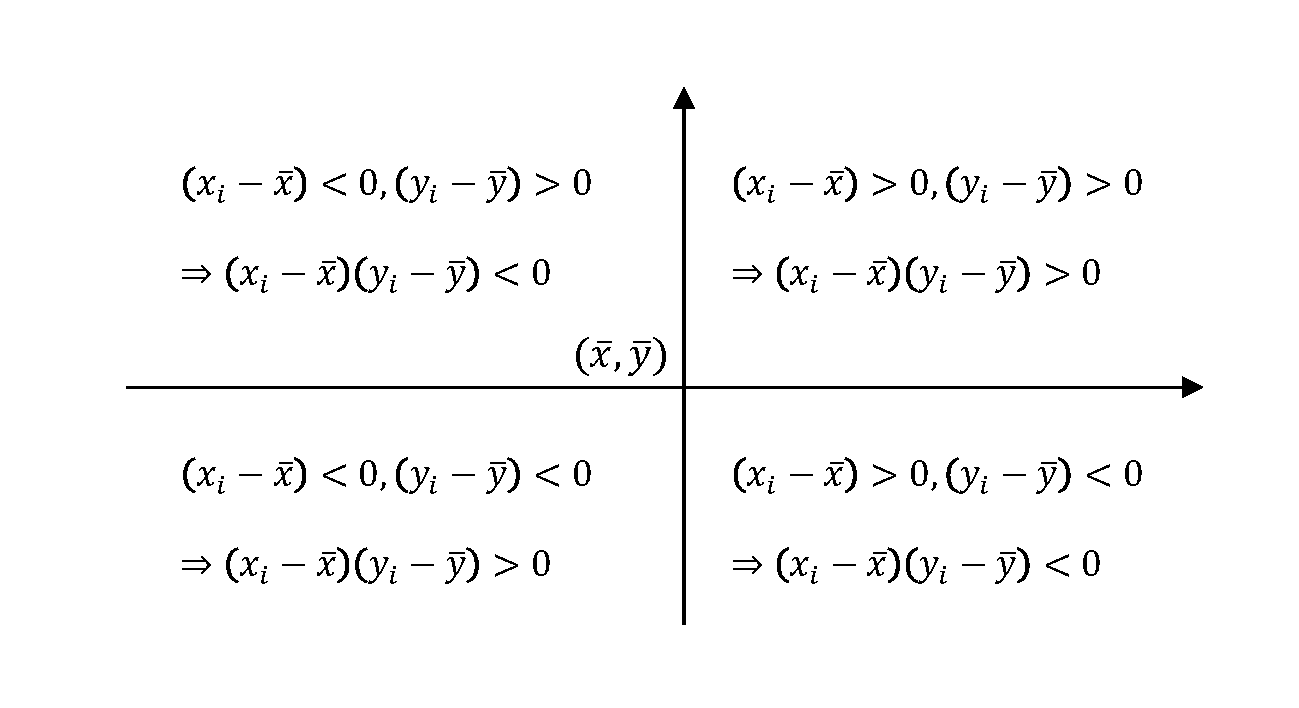
\includegraphics[width=0.8\linewidth]{7_Abbildungen/mvda_7_korrelationsterme} \end{center}

\center
\footnotesize

Häufige richtungsgleiche Abweichung der \(x_i\) und \(y_i\) von ihren
Mittelwerten \(\Rightarrow\) Positive Korrelation

Häufige richtungsungleiche Abweichung der \(x_i\) und \(y_i\) von ihren
Mittelwerten \(\Rightarrow\) Negative Korrelation

Keine häufigen richtungsgleichen oder -entgegengesetzten Abweichungen
\(\Rightarrow\) Keine Korrelation
\end{frame}

\begin{frame}{Korrelation}
\protect\hypertarget{korrelation-6}{}
\vspace{2mm}

Beispiele

\begin{center}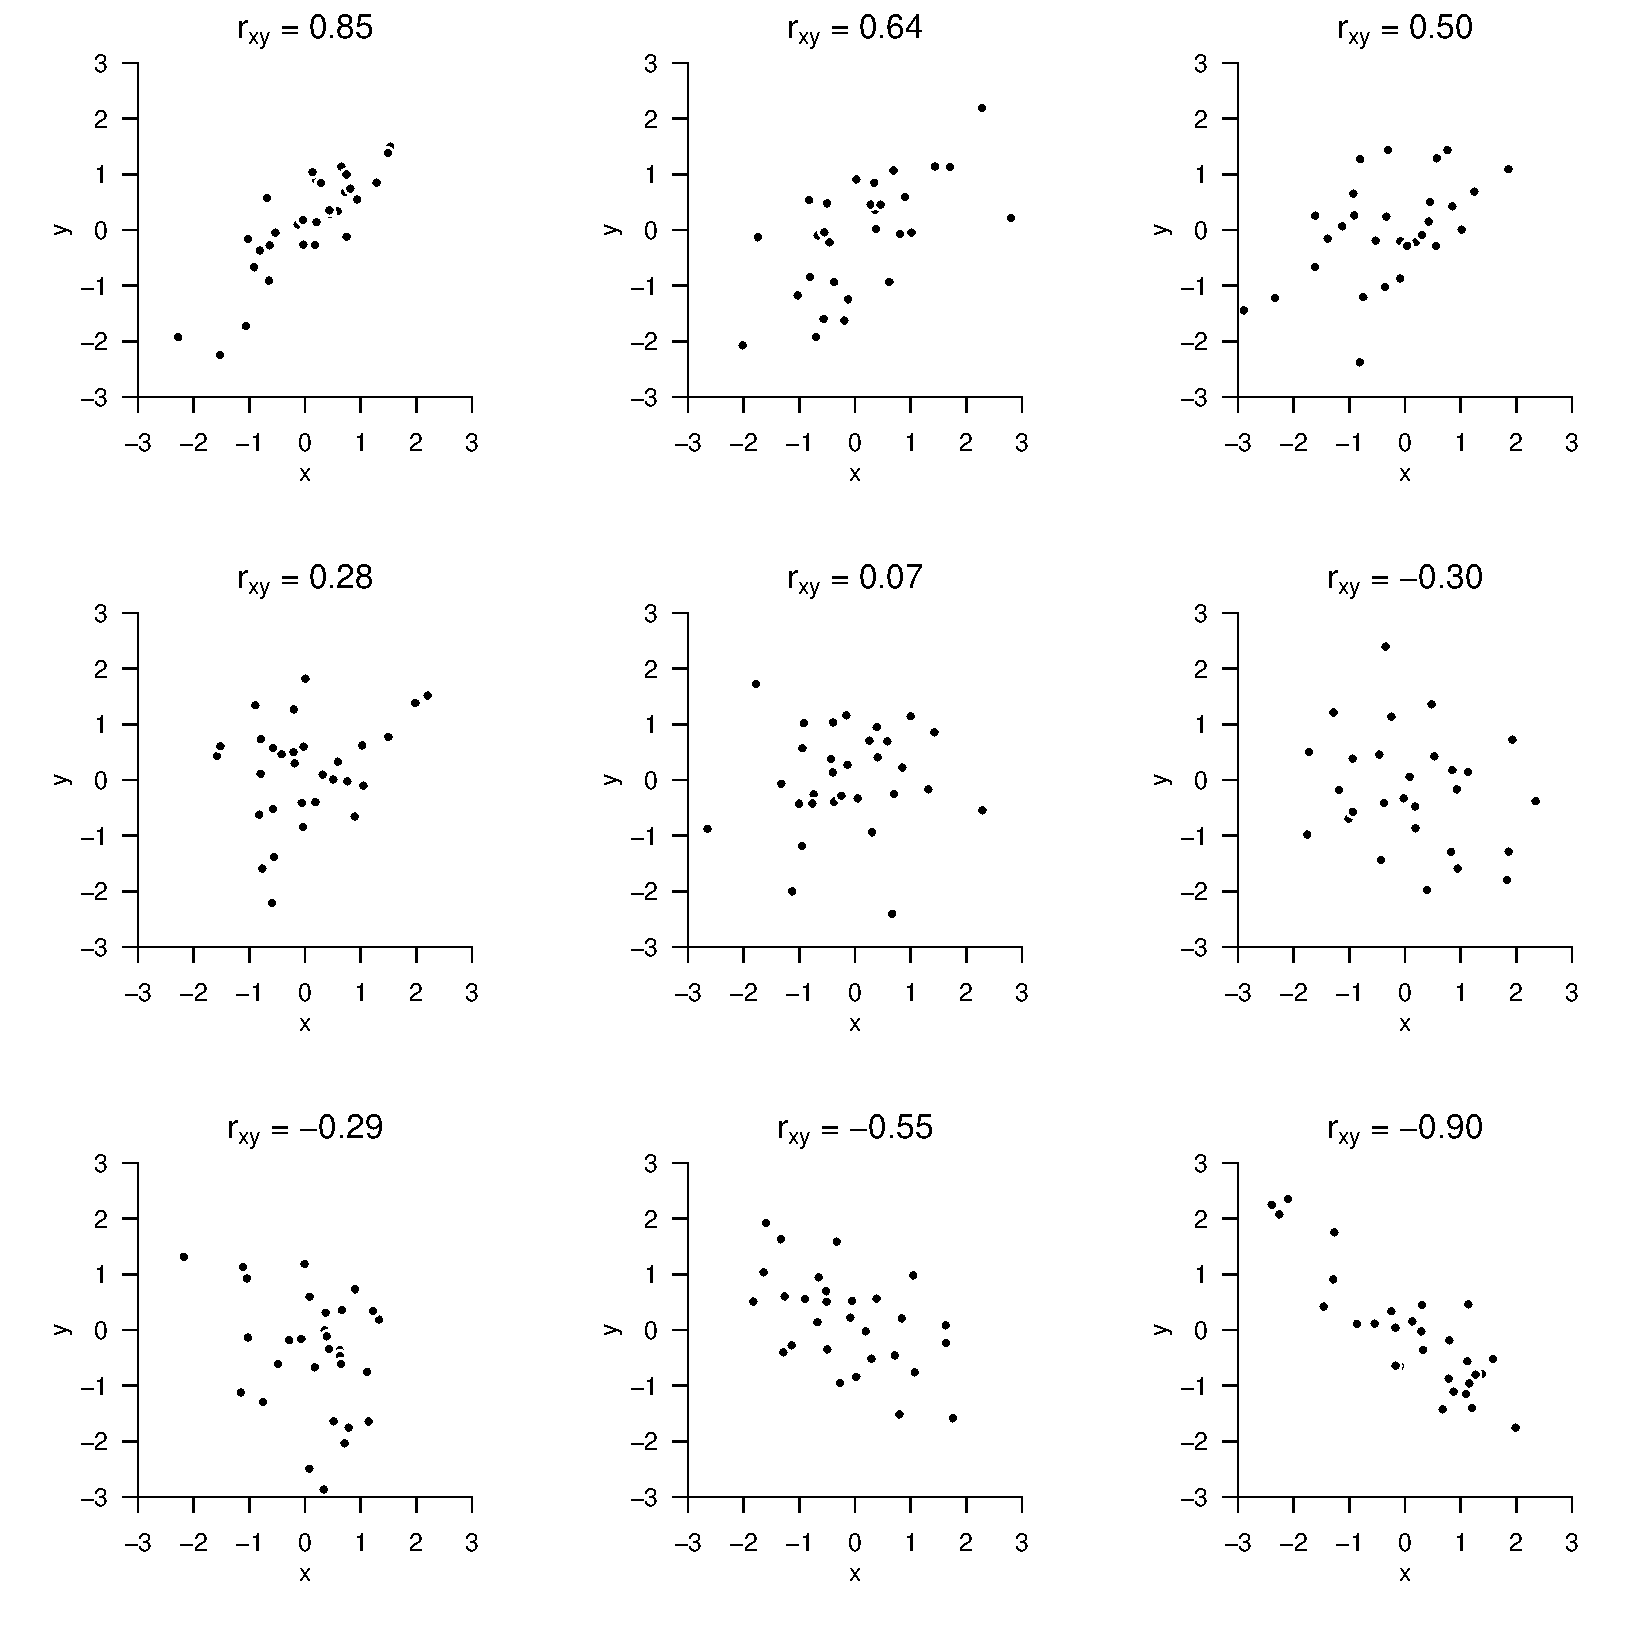
\includegraphics[width=0.6\linewidth]{7_Abbildungen/mvda_7_korrelationsbeispiele} \end{center}
\end{frame}

\begin{frame}{Korrelation}
\protect\hypertarget{korrelation-7}{}
Funktionale Abhängigkeiten und Stichprobenkorrelation

\vspace{1cm}

\begin{center}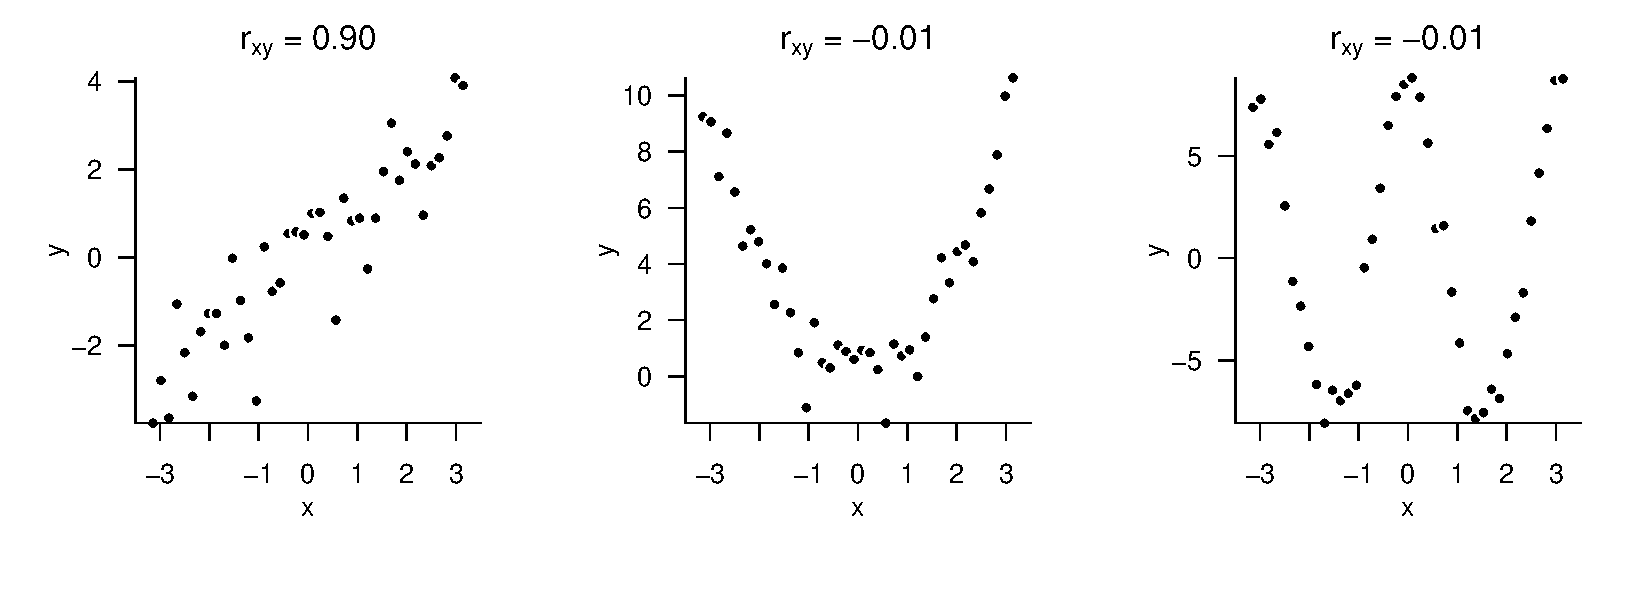
\includegraphics[width=1\linewidth]{7_Abbildungen/mvda_7_rlinearitaet} \end{center}
\vspace{-5mm}

\(\,\) \hspace{1cm} \(y_i = x_i + \varepsilon_i\) \hspace{1.9cm}
\(y_i = x_i^2 + \varepsilon_i\) \hspace{1.2cm}
\(y_i = 8 \cos(2x_i) + \varepsilon_i\)

\center

\(\quad\,\,\,\varepsilon_i \sim N(0,1)\)
\end{frame}

\begin{frame}{Korrelation}
\protect\hypertarget{korrelation-8}{}
\small
\begin{theorem}[Korrelation und linear-affine Abhängigkeit]
\justifying
\normalfont
$x$ und $y$ seien zwei Zufallsvariablen mit positiver Varianz. Dann besteht genau
dann eine lineare-affine Abhängigkeit der Form
\begin{equation}
y = \beta_0 + \beta_1x \mbox{ mit } \beta_0,\beta_1\in \mathbb{R}
\end{equation}
zwischen $x$ und $y$, wenn
\begin{equation}
\rho(x,y) = 1 \mbox{ oder } \rho(x,y) = -1.
\end{equation}
\end{theorem}

\footnotesize

Bemerkungen

\begin{itemize}
\tightlist
\item
  Für einen Beweis und eine vertiefte Diskussion verweisen wir auf die
  BSc Lehreinheiten.
\item
  Die linear-affine Abhängigkeit \(y = \beta_0 + \beta_1x\) impliziert
  eine linear-affine Abhängigkeit
  \(x = \tilde{\beta}_0 + \tilde{\beta}_1y\), denn \begin{equation}
  y = \beta_0 + \beta_1x
  \Leftrightarrow
  -\beta_0 + y = \beta_1x
  \Leftrightarrow
  x = -\frac{\beta_0}{\beta_1} + \frac{1}{\beta_1}y
  \Leftrightarrow
  x = \tilde{\beta}_0 + \tilde{\beta}_1 y
  \end{equation} mit \begin{equation}
  \tilde{\beta}_0 = -\frac{\beta_0}{\beta_1} \mbox{ und } \tilde{\beta}_1 = \frac{1}{\beta_1}.
  \end{equation}
\end{itemize}
\end{frame}

\begin{frame}{Korrelation}
\protect\hypertarget{korrelation-9}{}
\footnotesize
\begin{theorem}[Kovarianz und Korrelation bei linear-affinen Transformationen]
\justifying
\normalfont
$\xi$ und $\upsilon$ seien Zufallsvariablen und es seien $\alpha,\beta,\gamma,\delta \in \mathbb{R}$. 
Dann gelten
\begin{equation}
\mathbb{C}(\alpha\xi + \beta, \gamma\upsilon + \delta) = \alpha\beta\mathbb{C}(\xi,\upsilon)
\end{equation}
und
\begin{equation}
\rho(\alpha\xi + \beta, \gamma\upsilon + \delta) = \rho(\xi,\upsilon).
\end{equation}
\end{theorem}

Bemerkungen

\begin{itemize}
\tightlist
\item
  Wir benötigen diese Aussage im Kontext der Kanonischen
  Korrelationsanalyse.
\item
  Die Kovarianz zweier Zufallsvariablen ändert sich bei linear-affiner
  Transformation der Zufallsvariablen.
\item
  Die Korrelation zweier Zufallsvariablen ändert sich bei linear-affiner
  Transformation der Zufallsvariablen nicht.
\end{itemize}
\end{frame}

\begin{frame}{Korrelation}
\protect\hypertarget{korrelation-10}{}
\footnotesize

\underline{Beweis}

Es gilt zunächst \begin{align}
\begin{split}
\mathbb{C}(\alpha\xi+\beta,c\upsilon+d)
& = \mathbb{E}((\alpha\xi+\beta-\mathbb{E}(\alpha\xi+\beta))(\gamma\upsilon+\delta-\mathbb{E}(\gamma\upsilon+\delta)))    \\
& = \mathbb{E}((\alpha\xi+\beta-\alpha\mathbb{E}(\xi)-\beta)(\gamma\upsilon+\delta-\gamma\mathbb{E}(\gamma\upsilon)-\delta))   \\
& = \mathbb{E}(\alpha(\xi-\mathbb{E}(\xi))(\gamma(\upsilon -\gamma\mathbb{E}(\upsilon)))             \\
& = \mathbb{E}(\alpha\gamma((\xi-\mathbb{E}(\xi))(\upsilon -\gamma\mathbb{E}(\upsilon))))            \\
&  = \alpha\gamma\mathbb{C}(\xi,\upsilon)
\end{split}
\end{align} Also folgt \begin{align}
\begin{split}
\rho(\alpha\xi + \beta, \gamma\upsilon + \delta)
& = \frac{\mathbb{C}(\alpha\xi+\beta,\gamma\upsilon+\delta)}{\sqrt{\mathbb{V}(\alpha\xi+\beta)}\sqrt{\mathbb{V}(\gamma\upsilon+\delta)}} \\
& = \frac{\alpha\gamma\mathbb{C}(\xi,\upsilon)}{\sqrt{\alpha^2\mathbb{V}(\xi)}\sqrt{\gamma^2\mathbb{V}(\upsilon)}}     \\
& = \frac{\alpha\gamma\mathbb{C}(\xi,\upsilon)}{\alpha\mathbb{S}(\xi)c\mathbb{S}(\upsilon)}         \\
& = \frac{\mathbb{C}(\xi,\upsilon)}{\mathbb{S}(\xi)\mathbb{S}(\upsilon)}             \\
& = \rho(\xi,\upsilon).
\end{split}
\end{align}
\end{frame}

\begin{frame}{Korrelation}
\protect\hypertarget{korrelation-11}{}
Anwendungsszenario Kanonische Korrelation \vspace{3mm}

\begin{center}
\includegraphics[width=0.9\linewidth]{7_Abbildungen/mvda_7_beispielszenario_kanonische_korrelation} \end{center}
\end{frame}

\begin{frame}{Korrelation}
\protect\hypertarget{korrelation-12}{}
Beispieldatensatz Kanonische Korrelation

\footnotesize

\(i = 1,...,n\) Patient:innen

\center

\(y_{1i}\) BDI Score Reduktion, \(y_{2i}\) Glucocorticoid Reduktion,
\(x_{1i}\) Therapiedauer, \(x_{2i}\) Erfahrung Psychotherapeut:in,

\setstretch{1}

\begin{longtable}[]{@{}rrrr@{}}
\toprule()
x\_1i & x\_2i & y\_1i & y\_2i \\
\midrule()
\endhead
27.9 & 7.774 & 35.5 & 6.106 \\
15.3 & 9.347 & 25.0 & 3.961 \\
17.4 & 2.121 & 19.7 & 1.716 \\
21.5 & 6.517 & 28.8 & 2.617 \\
28.2 & 1.256 & 29.4 & 1.901 \\
14.0 & 2.672 & 17.2 & 0.872 \\
28.0 & 3.861 & 32.9 & 2.005 \\
28.9 & 0.134 & 28.3 & 4.073 \\
23.2 & 3.824 & 25.8 & 3.918 \\
22.6 & 8.697 & 31.3 & 3.770 \\
11.2 & 3.403 & 14.4 & 2.070 \\
14.1 & 4.821 & 18.4 & 1.999 \\
13.5 & 5.996 & 19.1 & 4.994 \\
23.7 & 4.935 & 28.0 & 2.566 \\
17.7 & 1.862 & 20.3 & 2.086 \\
25.4 & 8.274 & 34.8 & 4.445 \\
20.0 & 6.685 & 27.6 & 3.951 \\
24.4 & 7.942 & 31.9 & 3.851 \\
29.8 & 1.079 & 32.2 & 0.976 \\
17.6 & 7.237 & 24.6 & 1.944 \\
\bottomrule()
\end{longtable}
\end{frame}

\begin{frame}{Korrelation}
\protect\hypertarget{korrelation-13}{}
\textcolor{darkblue}{Grundzüge der Kanonischen Korrelationsanalyse}
\footnotesize

Die Datenvektoren \(x_{1i},...,x_{m_xi}, i = 1,...,n\) werden als u.i.v.
Realisierungen eines Zufallsvektors \(x\) interpretiert. Die
Datenvektoren \(y_{1i},...,y_{m_yi}, i = 1,...,n\) werden als u.i.v.
Realisierungen eines Zufallsvektors \(y\) interpretiert.

Die ``erste kanonische Korrelation'' ist die maximale Korrelation von
Linearkombinationen von \(x\) und \(y\); wir bezeichnen die
Linearkombinationen von \(x\) und \(y\) mit Vektoren
\(a \in \mathbb{R}^{m_x}\) und \(b \in \mathbb{R}^{m_y}\) mit
\begin{equation}
\xi      = a^Tx = a_1x_1 + \cdots + a_{m_x}x_{m_x}
\mbox{ und }
\upsilon = b^Ty = b_1y_1 + \cdots + b_{m_y}y_{m_y}
\end{equation} \(\xi\) und \(\upsilon\) sind dann als
Linearkombinationen von Zufallsvariablen selbst Zufallsvariablen; Die
Korrelation von \(\xi\) und \(\upsilon\) bezeichnen wir mit
\(\rho(\xi,\upsilon)\)

Wenn die Zufallsvektoren \(x\) als unabhängige Variable und \(y\) als
abhängige Variable interpretiert werden, dann kann \(\xi= a^Tx\) als
``bester Prädiktor'' und \(\upsilon = b^Ty\) als ``am besten
prädizierbares Kriterium'' interpretiert werden. Kanonische
Korrelationsanalyse fragt damit nach Parametern
\(a \in \mathbb{R}^{m_x}\) und \(b\in \mathbb{R}^{m_y}\) für die
\(\rho(\xi,\upsilon)\) maximal ist.

Für Skalare \(\alpha,\beta\in \mathbb{R}\) sind die Korrelationen
\(\rho(a^Tx,b^Ty)\) und \(\rho((\alpha a^T)x,(\beta b^T)y)\) allerdings
identisch (siehe unten). Man sucht deshalb Parameter
\(a \in \mathbb{R}^{m_x}\) und \(b\in \mathbb{R}^{m_y}\) für die
\(\rho(\xi,\upsilon)\) maximal ist und für die \(a^Tx\) und \(b^Ty\)
jeweils eine Varianz von 1 haben, also
\(\mathbb{V}(\xi) = \mathbb{V}(\upsilon) = 1\) gilt.

Anders ausgedrückt: Die Varianzen von \(a^Tx\) und \(b^Ty\) und die
Varianzen von Linearkombinationen von \(x\) und \(y\) mit beliebigen
skalaren Vielfachen von \(a\) und \(b\) sind im Sinne der ersten Aussage
des Theorems zur Kovarianz und Korrelation bei linear-affinen
Transformationen verschieden.
\end{frame}

\begin{frame}{Korrelation}
\protect\hypertarget{korrelation-14}{}
\textcolor{darkblue}{Grundzüge der Kanonischen Korrelationsanalyse}

\footnotesize

Insbesondere gilt einen \(m_x\)-dimensionalen Zufallsvektoren \(x\) und
einen \(m_y\)-dimensionalen Zufallsvektor \(y\),
\(a \in \mathbb{R}^{m_x},b \in \mathbb{R}^{m_y}\),
\(\alpha,\beta \in \mathbb{R}\) und die Linearkombinationen
\(\xi := a^Tx\) und \(\upsilon := b^Ty\) basierend auf dem Theorems zur
Kovarianz und Korrelation bei linear-affinen allerdings auch, dass
\begin{equation*}
\rho(\xi,\upsilon) = \rho(\alpha\xi,\beta\upsilon)   
\Leftrightarrow
\rho(a^Tx, b^Ty)   = \rho(\alpha(a^Tx),\beta(b^Ty))  
\Leftrightarrow
\rho(a^Tx, b^Ty)   = \rho((\alpha a^T)x),(\beta b^T)y).
\end{equation*} Die Korrelation von \(a^Tx\) und \(b^Ty\) und die
Korrelationen von Linearkombinationen von \(x\) und \(y\) mit beliebigen
skalaren Vielfachen von \(a\) und \(b\) sind also gleich.

Zur Entwicklung der Kanonischen Korrelationsanalyse folgen wir Mardia,
Kent, and Bibby (1979), Kapitel 10. Dabei werden die Zufallsvektoren
\(x\) und \(y\) in einem Zufallsvektor \begin{equation}
z := \begin{pmatrix} x \\ y \end{pmatrix}
\end{equation} zusammengefasst, für den wir durchgängig annehmen, dass
\(\mathbb{E}(z) = 0_{m}\) mit \(m = m_x + m_y\). Dies entspricht auf der
Anwendungsebene der Subtraktion des Stichprobenmittels von den
beobachteten Daten vor Durchführung der Kanonischen Korrelationsanalyse

Der mathematische Fokus der Entwicklung nach Mardia, Kent, and Bibby
(1979), Kapitel 10 ist auf der Kovarianzmatrix \(\mathbb{C}(z)\).
Speziell ergeben sich die Kovarianzen von Linearkombinationen von \(x\)
und \(y\) aus Matrixprodukten von \(\mathbb{C}(z)\) und es können einige
Matrixtheoreme, dieim Folgenden diskutiert werden, auf diese
Matrixprodukte angewendet werden. Generell wird in der Entwicklung nach
Mardia, Kent, and Bibby (1979), Kapitel 10 ein restringierter
Optimierungsansatz mithilfe der Lagrangefunktion zugunsten der
Eigenanalyse von Matrixprodukten supprimiert. Für die Entwicklung mit
einem Lagrangeansatz, siehe zum Beispiel Anderson (2003), Kapitel 12.
\end{frame}

\begin{frame}{}
\protect\hypertarget{section-5}{}
\setstretch{2.5}
\vfill
\large

Korrelation

\textbf{Algebraische Grundlagen}

Wahrscheinlichkeitstheoretische Grundlagen

Modellformulierung

Modellschätzung

Selbstkontrollfragen \vfill
\end{frame}

\begin{frame}{Algebraische Grundlagen}
\protect\hypertarget{algebraische-grundlagen}{}
\footnotesize
\begin{definition}[Symmetrische Quadratwurzel einer Matrix]
\justifying
$A \in \mathbb{R}^{m \times m}$ sei eine invertierbare symmetrische Matrix mit
positiven Eigenwerten. Dann sind für $r \in \mathbb{N}^0$ und $s \in \mathbb{N}$
die rationalen Potenzen von $A$ einer orthonormalen Matrix $Q \in \mathbb{R}^{m \times m}$
der Eigenvektoren von $A$ und einer Diagonalmatrix  $\Lambda = \mbox{diag}(\lambda_i) \in \mathbb{R}^{m \times m}$
der zugehörigen Eigenwerte $\lambda_1,...,\lambda_m$ von $A$ definiert als
\begin{equation}
A^{r/s} = Q \Lambda^{r/s} Q^T \mbox{ mit } \Lambda^{r/s} = \mbox{diag}\left(\lambda_i^{r/s}\right).
\end{equation}
Der Spezialfall $r:= 1, s := 2$ wird als symmetrische Quadratwurzel von $A$ bezeichnet
und hat die Form
\begin{equation}
A^{1/2} = Q\Lambda^{1/2}Q^T \mbox{ mit } \Lambda^{1/2} = \mbox{diag}\left(\lambda_i^{1/2}\right).
\end{equation}
\end{definition}
\setstretch{1}

Bemerkungen

\begin{itemize}
\tightlist
\item
  Offenbar gilt \begin{equation}
  \left(A^{1/2} \right)^2 = Q\Lambda^{1/2}Q^TQ\Lambda^{1/2}Q^T = Q\Lambda^{1/2}\Lambda^{1/2}Q^T =  Q\Lambda Q^T = A.
  \end{equation}
\item
  Weiterhin gilt \begin{equation}
  \left(A^{-1/2} \right)^2 = Q\Lambda^{-1/2}Q^TQ\Lambda^{-1/2}Q^T = Q\Lambda^{-1}Q^T = A^{-1}.
  \end{equation} Die vorletzte Gleichung mag überraschen, aber es gilt
  ja zum Beispiel \begin{equation}
  4^{-1/2}\cdot 4^{-1/2} = \frac{1}{\sqrt{4}}\cdot\frac{1}{\sqrt{4}} = \frac{1}{4} = 4^{-1}.
  \end{equation}
\end{itemize}
\end{frame}

\begin{frame}[fragile]{Algebraische Grundlagen}
\protect\hypertarget{algebraische-grundlagen-1}{}
\footnotesize
\begin{theorem}[Eigenwerte und Eigenvektoren von Matrixprodukten]
\justifying
\normalfont
Für $A \in \mathbb{R}^{n \times m}$ und $B \in \mathbb{R}^{m \times n}$ sind
die Eigenwerte von $AB \in \mathbb{R}^{n \times n}$ und $BA \in \mathbb{R}^{m \times m}$
gleich. Weiterhin gilt, dass für einen Eigenvektor $v$ zu einem von Null
verschiedenen Eigenwert $\lambda$ von $AB$ $w := Bv$ ein Eigenvektor von $BA$ ist.
\end{theorem}

Bemerkungen

\begin{itemize}
\tightlist
\item
  Für einen Beweis siehe Mardia, Kent, and Bibby (1979), S. 468.
\end{itemize}

\vspace{1mm}
\tiny
\setstretch{1.2}

\begin{Shaded}
\begin{Highlighting}[]
\NormalTok{A   }\OtherTok{=} \FunctionTok{matrix}\NormalTok{(}\DecValTok{1}\SpecialCharTok{:}\DecValTok{6}\NormalTok{, }\AttributeTok{nrow =} \DecValTok{2}\NormalTok{,  }\AttributeTok{byrow =}\NormalTok{ T)           }\CommentTok{\# Matrix A \textbackslash{}in \textbackslash{}mathbb\{R\}\^{}\{2 x 3\}}
\NormalTok{B   }\OtherTok{=} \FunctionTok{matrix}\NormalTok{(}\DecValTok{1}\SpecialCharTok{:}\DecValTok{6}\NormalTok{, }\AttributeTok{ncol =} \DecValTok{2}\NormalTok{,  }\AttributeTok{byrow =}\NormalTok{ T)           }\CommentTok{\# Matrix B \textbackslash{}in \textbackslash{}mathbb\{R\}\^{}\{3 x 2\}}
\NormalTok{EAB }\OtherTok{=} \FunctionTok{eigen}\NormalTok{(A }\SpecialCharTok{\%*\%}\NormalTok{ B)                              }\CommentTok{\# Eigenanalyse von AB \textbackslash{}in \textbackslash{}mathbb\{R\}\^{}\{2 \textbackslash{}times 2\}}
\NormalTok{EBA }\OtherTok{=} \FunctionTok{eigen}\NormalTok{(B }\SpecialCharTok{\%*\%}\NormalTok{ A)                              }\CommentTok{\# Eigenanalyse von BA \textbackslash{}in \textbackslash{}mathbb\{R\}\^{}\{3 \textbackslash{}times 3\}}
\NormalTok{w   }\OtherTok{=}\NormalTok{ B }\SpecialCharTok{\%*\%}\NormalTok{ EAB}\SpecialCharTok{$}\NormalTok{vectors[,}\DecValTok{1}\NormalTok{]                       }\CommentTok{\# Eigenvektor von BA}
\FunctionTok{cat}\NormalTok{(}\StringTok{"Eigenwerte von AB :"}\NormalTok{  , EAB}\SpecialCharTok{$}\NormalTok{values[}\DecValTok{1}\SpecialCharTok{:}\DecValTok{2}\NormalTok{],}
    \StringTok{"}\SpecialCharTok{\textbackslash{}n}\StringTok{Eigenwerte von BA :"}\NormalTok{, EBA}\SpecialCharTok{$}\NormalTok{values[}\DecValTok{1}\SpecialCharTok{:}\DecValTok{2}\NormalTok{],}
    \StringTok{"}\SpecialCharTok{\textbackslash{}n}\StringTok{BAw mit w = Bv    :"}\NormalTok{, B }\SpecialCharTok{\%*\%}\NormalTok{ A }\SpecialCharTok{\%*\%}\NormalTok{ w,}
    \StringTok{"}\SpecialCharTok{\textbackslash{}n}\StringTok{lw mit w = Bv     :"}\NormalTok{, EBA}\SpecialCharTok{$}\NormalTok{values[}\DecValTok{1}\NormalTok{] }\SpecialCharTok{*}\NormalTok{ w)}
\end{Highlighting}
\end{Shaded}

\begin{verbatim}
> Eigenwerte von AB : 85.6 0.421 
> Eigenwerte von BA : 85.6 0.421 
> BAw mit w = Bv    : -191 -417 -642 
> lw mit w = Bv     : -191 -417 -642
\end{verbatim}
\end{frame}

\begin{frame}[fragile]{Algebraische Grundlagen}
\protect\hypertarget{algebraische-grundlagen-2}{}
\footnotesize
\begin{theorem}[Eigenwert und Eigenvektor eines Matrixvektorprodukts]
\justifying
\normalfont
Für $A \in \mathbb{R}^{n \times m}, B \in \mathbb{R}^{p \times n}, a \in \mathbb{R}^m$
und $b \in \mathbb{R}^p$ gilt, dass der einzige von Null verschiedene Eigenwert von
$Aab^TB \in \mathbb{R}^{n \times n}$ gleich $b^T BAa$ mit zugehörigem Eigenvektor $Aa$ ist.
\end{theorem}

Bemerkungen

\begin{itemize}
\tightlist
\item
  Für einen Beweis siehe Mardia, Kent, and Bibby (1979), S. 468.
\end{itemize}

\vspace{1mm}
\tiny
\setstretch{1.2}
\vspace{1mm}
\tiny
\setstretch{1.2}

\begin{Shaded}
\begin{Highlighting}[]
\NormalTok{A      }\OtherTok{=} \FunctionTok{matrix}\NormalTok{(}\DecValTok{1}\SpecialCharTok{:}\DecValTok{6}\NormalTok{, }\AttributeTok{nrow =} \DecValTok{2}\NormalTok{,  }\AttributeTok{byrow =}\NormalTok{ T)     }\CommentTok{\# Matrix A \textbackslash{}in \textbackslash{}mathbb\{R\}\^{}\{2 x 3\}}
\NormalTok{B      }\OtherTok{=} \FunctionTok{matrix}\NormalTok{(}\DecValTok{1}\SpecialCharTok{:}\DecValTok{8}\NormalTok{, }\AttributeTok{ncol =} \DecValTok{2}\NormalTok{,  }\AttributeTok{byrow =}\NormalTok{ T)     }\CommentTok{\# Matrix B \textbackslash{}in \textbackslash{}mathbb\{R\}\^{}\{4 x 2\}}
\NormalTok{a      }\OtherTok{=} \FunctionTok{matrix}\NormalTok{(}\DecValTok{1}\SpecialCharTok{:}\DecValTok{3}\NormalTok{, }\AttributeTok{nrow =} \DecValTok{3}\NormalTok{,  }\AttributeTok{byrow =}\NormalTok{ T)     }\CommentTok{\# Vektor a \textbackslash{}in \textbackslash{}mathbb\{R\}\^{}\{3 x 1\}}
\NormalTok{b      }\OtherTok{=} \FunctionTok{matrix}\NormalTok{(}\DecValTok{1}\SpecialCharTok{:}\DecValTok{4}\NormalTok{, }\AttributeTok{nrow =} \DecValTok{4}\NormalTok{,  }\AttributeTok{byrow =}\NormalTok{ T)     }\CommentTok{\# Vektor b \textbackslash{}in \textbackslash{}mathbb\{R\}\^{}\{4 x 1\}}
\NormalTok{EAabTB }\OtherTok{=} \FunctionTok{eigen}\NormalTok{(A }\SpecialCharTok{\%*\%}\NormalTok{ a }\SpecialCharTok{\%*\%} \FunctionTok{t}\NormalTok{(b) }\SpecialCharTok{\%*\%}\NormalTok{ B)         }\CommentTok{\# Eigenanalyse von Aab\^{}TB \textbackslash{}in \textbackslash{}mathbb\{R\}\^{}\{4 x 4\}}
\FunctionTok{cat}\NormalTok{(}\StringTok{"Eigenwerte von AabTB :"}\NormalTok{, EAabTB}\SpecialCharTok{$}\NormalTok{values,}
    \StringTok{"}\SpecialCharTok{\textbackslash{}n}\StringTok{bTBAa                :"}\NormalTok{, }\FunctionTok{t}\NormalTok{(b) }\SpecialCharTok{\%*\%}\NormalTok{ B }\SpecialCharTok{\%*\%}\NormalTok{ A }\SpecialCharTok{\%*\%}\NormalTok{ a,}
    \StringTok{"}\SpecialCharTok{\textbackslash{}n}\StringTok{Aa                   :"}\NormalTok{, A }\SpecialCharTok{\%*\%}\NormalTok{ a,}
    \StringTok{"}\SpecialCharTok{\textbackslash{}n}\StringTok{(AabTB)Aa            :"}\NormalTok{,(A }\SpecialCharTok{\%*\%}\NormalTok{ a }\SpecialCharTok{\%*\%} \FunctionTok{t}\NormalTok{(b) }\SpecialCharTok{\%*\%}\NormalTok{ B) }\SpecialCharTok{\%*\%}\NormalTok{ A }\SpecialCharTok{\%*\%}\NormalTok{ a,            }\CommentTok{\# Mv}
    \StringTok{"}\SpecialCharTok{\textbackslash{}n}\StringTok{(bTBAa)Aa            :"}\NormalTok{,}\FunctionTok{as.vector}\NormalTok{((}\FunctionTok{t}\NormalTok{(b) }\SpecialCharTok{\%*\%}\NormalTok{ B }\SpecialCharTok{\%*\%}\NormalTok{ A }\SpecialCharTok{\%*\%}\NormalTok{ a)) }\SpecialCharTok{*}\NormalTok{ (A }\SpecialCharTok{\%*\%}\NormalTok{ a)) }\CommentTok{\# = \textbackslash{}lambda v}
\end{Highlighting}
\end{Shaded}

\begin{verbatim}
> Eigenwerte von AabTB : 2620 0 
> bTBAa                : 2620 
> Aa                   : 14 32 
> (AabTB)Aa            : 36680 83840 
> (bTBAa)Aa            : 36680 83840
\end{verbatim}
\end{frame}

\begin{frame}{Algebraische Grundlagen}
\protect\hypertarget{algebraische-grundlagen-3}{}
\footnotesize
\begin{theorem}[Maximierung quadratischer Formen mit Nebenbedingungen]
\justifying
\normalfont
$A \in \mathbb{R}^{m \times m}, B \in \mathbb{R}^{m \times m} \mbox{ p.d.}$
seien symmetrische Matrizen und $\lambda_1$ sei der größte Eigenwert von $B^{-1}A$
mit assoziertem Eigenvektor $v_1 \in \mathbb{R}^m$. Dann ist $\lambda_1$ eine Lösung des
Optimierungsproblems
\begin{equation}\label{eq:opt_1}
\max_{x} x^TAx \mbox{ unter der Nebenbedingung } x^TBx = 1.
\end{equation}
\end{theorem}

Bemerkungen

\begin{itemize}
\tightlist
\item
  Das Theorem ist direkt durch die kanonische Korrelationsanalyse
  motiviert.
\item
  \(\max_{x} f(x)\) ist das Maximum einer Funktion \(f\), also der Wert
  der Funktion an der Maximumstelle \(x\)
\item
  \(\argmax_{x} f(x)\) ist die Maximumstelle einer Funktion, also ein
  Wert in der Definitionsmenge von \(f\).
\item
  Nach Wortlaut des Theorems gilt also für die Funktion \begin{equation}
  f : \mathbb{R}^m \to \mathbb{R}, x \mapsto f(x) := x^TAx,
  \end{equation} dass \begin{equation}
  v_1 = \argmax_{x} x^TAx \mbox{ unter der Nebenbedingung } x^TBx = 1
  \end{equation} und dass \begin{equation}
  \lambda_1 = \max_{x} x^TAx \mbox{ unter der Nebenbedingung } x^TBx = 1.
  \end{equation}
\end{itemize}
\end{frame}

\begin{frame}{Algebraische Grundlagen}
\protect\hypertarget{algebraische-grundlagen-4}{}
\footnotesize

\underline{Beweis}

\(B^{1/2}\) sei die symmetrische Quadratwurzel von \(B\) und es sei
\begin{equation}
y := B^{1/2}x \Leftrightarrow x = B^{-1/2}y
\end{equation} Dann kann mit der symmetrischen Matrix \begin{equation}
K := B^{-1/2}AB^{-1/2} \in \mathbb{R}^{m \times m}
\end{equation} das Optimierungsproblem \eqref{eq:opt_1} geschrieben
werden als \begin{equation}\label{eq:opt_2}
\max_{y} y^T K y
\mbox{ unter der Nebenbedingung }
y^Ty = 1.
\end{equation} Dies gilt, weil \begin{equation}
\max_{x} x^TAx
\Leftrightarrow
\max_{y} \left(B^{-1/2}y\right)^TA\left(B^{-1/2}y\right)
\Leftrightarrow
\max_{y} y^TB^{-1/2}AB^{-1/2}y
\Leftrightarrow
\max_{y} y^TKy
\end{equation} und \begin{equation}
x^TBx = 1
\Leftrightarrow y^T B^{-1/2}BB^{-1/2}y = 1
\Leftrightarrow y^Ty = 1.
\end{equation} Weil \(K\) eine symmetrische Matrix ist, existiert die
Orthonormalzerlegung (vgl. (2) Matrizen) \begin{equation}
K = Q\Lambda Q^T,
\end{equation} wobei die Spalten der orthogonalen Matrix \(Q\) die
Eigenvektoren von \(K\) und die Diagonalemente von \(\Lambda\) die
zugehörigen Eigenwerte von \(K\) sind.
\end{frame}

\begin{frame}{Algebraische Grundlagen}
\protect\hypertarget{algebraische-grundlagen-5}{}
\footnotesize

\underline{Beweis (fortgeführt)}

Mit der orthogonalen Matrix \(Q\) aus obiger Orthornomalzerlegung sei
nun \begin{equation}
z := Q^Ty \Leftrightarrow y := Qz.
\end{equation} Dann kann das Optimierungsproblem \eqref{eq:opt_2}
geschrieben werden als \begin{equation}\label{eq:opt_3}
\max_{z} \sum_{i = 1}^m \lambda_i z_i^2 \mbox{ unter der Nebenbedingung } z^Tz = 1,
\end{equation} weil \begin{equation}
\max_{y} y^TKy
\Leftrightarrow
\max_{z} (Qz)^TK(Qz)
\Leftrightarrow
\max_{z} z^TQ^TQ\Lambda Q^TQz
\Leftrightarrow
\max_{z} z^T\Lambda z
\Leftrightarrow
\max_{z} \sum_{i=1}^m \lambda_i z_i^2
\end{equation} und \begin{equation}
y^Ty = 1
\Leftrightarrow
(Qz)^T Qz = 1
\Leftrightarrow
z^T Q^TQz = 1
\Leftrightarrow
z^T z = 1.
\end{equation}
\end{frame}

\begin{frame}{Algebraische Grundlagen}
\protect\hypertarget{algebraische-grundlagen-6}{}
\footnotesize

\underline{Beweis (fortgeführt)}

Die Eigenwerte von \(K\) seien nun absteigend sortiert, also
\(\lambda_1 \ge \cdots \ge \lambda_m\). Dann gilt für das
Optimierungsproblem \eqref{eq:opt_3}, dass \begin{equation}
\max_{z} \sum_{i = 1}^m \lambda_i z_i^2 \le \lambda_1,
\end{equation} weil \begin{equation}
\max_{z} \sum_{i = 1}^m \lambda_i z_i^2
\le
\max_{z} \sum_{i = 1}^m \lambda_1 z_i^2
=
\lambda_1 \max_{z} \sum_{i = 1}^m z_i^2
=
\lambda_1
\end{equation} wobei sich die letzte Gleichung aus der Nebenbedingung
\(z^Tz=1\) ergibt. Schließlich gilt \begin{equation}
\max_{z} \sum_{i = 1}^m \lambda_i z_i^2  = \lambda_1,
\end{equation} für \(z := e_1 = (1,0,...,0)^T\). Zusammenfassend heißt
das, dass \(z = e_1\) eine Lösung des Optimierungsproblem
\eqref{eq:opt_3} ist und das \(\lambda_1\) das entsprechende Maximum
ist.
\end{frame}

\begin{frame}{Vorbemerkungen}
\protect\hypertarget{vorbemerkungen}{}
\footnotesize

\underline{Beweis (fortgeführt)}

Damit ergibt sich aber sofort, dass dann \begin{equation}
y = Qz = Qe_1 =  q_1 \mbox{ und } x = B^{-1/2}q_1
\end{equation} Lösungen der äquivalenten Optimierungsprobleme
\eqref{eq:opt_2} und \eqref{eq:opt_1}, respektive, sind. Nach
Konstruktion ist \(q_1\) ein Eigenvektor von \(B^{-1/2}AB^{-1/2}\) und
nach obigem Theorem zu Eigenwerten und Eigenvektoren von Matrixprodukten
damit auch ein Eigenvektor von \begin{equation}
B^{-1/2}B^{-1/2}A = B^{-1}A
\end{equation} und die zugehörigen Eigenwerte sind gleich. Damit aber
folgt, dass der größte Eigenwert von \(B^{-1}A\) und sein assoziierter
Eigenvektor eine Lösung von \begin{equation}
\max_{x} x^TAx \mbox{ unter der Nebenbedingung } x^TBx = 1.
\end{equation} ist. \(\hfill\Box\)
\end{frame}

\begin{frame}{}
\protect\hypertarget{section-6}{}
\setstretch{2.5}
\vfill
\large

Korrelation

Algebraische Grundlagen

\textbf{Wahrscheinlichkeitstheoretische Grundlagen}

Modellformulierung

Modellschätzung

Selbstkontrollfragen \vfill
\end{frame}

\begin{frame}{Wahrscheinlichkeitstheoretische Grundlagen}
\protect\hypertarget{wahrscheinlichkeitstheoretische-grundlagen}{}
\footnotesize
\begin{theorem}[Kovarianzmatrizen von Zufallsvektoren]
\normalfont
\justifying
Es seien
\begin{equation}
z = \begin{pmatrix} x \\ y\end{pmatrix}
\mbox{ mit }
\mathbb{E}(z)  := 0_m
\end{equation}
ein $m_x + m_y$-dimensionaler Zufallsvektor und sein Erwartungswertvektor,
respektive. Dann kann die $m \times m$ Kovarianzmatrix  $z$ geschrieben werden als
\begin{equation}
\mathbb{C}(z) =
\begin{pmatrix}
\Sigma_{xx} & \Sigma_{xy} \\
\Sigma_{yx} & \Sigma_{yy} \\
\end{pmatrix}
\in \mathbb{R}^{m \times m}
\end{equation}
wobei
\begin{align}
\begin{split}
\Sigma_{xx} & := \mathbb{E}\left(xx^T\right) \in \mathbb{R}^{m_x \times m_x}\\
\Sigma_{xy} & := \mathbb{E}\left(xy^T\right) \in \mathbb{R}^{m_x \times m_y}\\
\Sigma_{yx} & := \mathbb{E}\left(yx^T\right) \in \mathbb{R}^{m_y \times m_x}\\
\Sigma_{yy} & := \mathbb{E}\left(yy^T\right) \in \mathbb{R}^{m_x \times m_y}
\end{split}
\end{align}
\end{theorem}
\end{frame}

\begin{frame}{Wahrscheinlichkeitstheoretische Grundlagen}
\protect\hypertarget{wahrscheinlichkeitstheoretische-grundlagen-1}{}
\footnotesize

\underline{Beweis}

\renewcommand{\arraystretch}{1.2}

Nach Definition der Kovarianzmatrix eines Zufallsvektors gilt
\begin{align}
\begin{split}
\mathbb{C}(z)
& = \mathbb{E}\left((z - \mathbb{E}(z))(z - \mathbb{E}(z))^T \right) \\
& = \mathbb{E}\left((z - 0_m)(z - 0_m)^T \right) \\
& = \mathbb{E}\left(zz^T\right)\\
& = \mathbb{E}\left(\begin{pmatrix} x \\ y \end{pmatrix} \begin{pmatrix} x^T & y^T \end{pmatrix} \right) \\
& = \mathbb{E}\left(\begin{pmatrix} xx^T & xy^T \\ yx^T & yy^T \end{pmatrix}\right)
\\
& =
\begin{pmatrix}
\mathbb{E}\left(xx^T\right) & \mathbb{E}\left(xy^T\right) \\
\mathbb{E}\left(yx^T\right) & \mathbb{E}\left(yy^T\right)
\end{pmatrix}
\\
& =
\begin{pmatrix}
\Sigma_{xx} & \Sigma_{xy} \\
\Sigma_{yx} & \Sigma_{yy} \\
\end{pmatrix}
\end{split}
\end{align} \(\hfill\Box\)
\end{frame}

\begin{frame}{Modellformulierung}
\protect\hypertarget{modellformulierung}{}
\footnotesize
\begin{theorem}[Linearkombinationen von Zufallsvektorpartitionen]
\justifying
\normalfont
Es sei
\begin{equation}
z = \begin{pmatrix} x \\ y \end{pmatrix}
\mbox{ mit }
\mathbb{E}(x) = 0_m
\mbox{ und }
\mathbb{C}(z) =
\begin{pmatrix}
\Sigma_{xx} & \Sigma_{xy} \\
\Sigma_{yx} & \Sigma_{yy} \\
\end{pmatrix}
\end{equation}
ein $m$-dimensionaler partitionierter Zufallsvektor sowie sein
Erwartungswertvektor und seine Kovarianzmatrix, respektive. Weiterhin seien für
$a \in \mathbb{R}^{m_x}$ und $b\in\mathbb{R}^{m_y}$
die Zufallsvariablen
\begin{equation}
\xi := a^T x \mbox{ und } \upsilon := b^T y
\end{equation}
als Linearkombinationen der Komponenten von $x$ und $y$ definiert.
Dann gelten
\begin{itemize}
\item[(1)] $\mathbb{V}(\xi) = a^T\Sigma_{xx}a$
\item[(2)] $\mathbb{V}(\upsilon) = b^T\Sigma_{yy}b$
\item[(2)] $\rho(\xi,\upsilon) = a^T \Sigma_{xy}b$, wenn  $\mathbb{V}(\xi) = 1$ und $\mathbb{V}(\upsilon) = 1$.
\end{itemize}
\end{theorem}

Bemerkungen

\begin{itemize}
\tightlist
\item
  Die Varianz der Zufallsvariable \(a^Tx\) ergibt sich als ``doppelte
  Linearkombination'' von \(\Sigma_{xx}\).
\item
  Die Varianz der Zufallsvariable \(b^Ty\) ergibt sich als ``doppelte
  Linearkombination'' von \(\Sigma_{yy}\).
\item
  Die Korrelation der Zufallsvariablen \(a^Tx\) und \(b^Ty\) ergibt sich
  ``doppellte Linearkombination'' von \(\Sigma_{xy}\).
\end{itemize}
\end{frame}

\begin{frame}{Modellformulierung}
\protect\hypertarget{modellformulierung-1}{}
\footnotesize

\underline{Beweis von (1) und (2)}

Wir betrachten zunächst die Varianz von \(\xi\). Mit dem
Varianzverschiebungssatz (vgl.
\href{https://youtu.be/613-3a1Pyyg}{\textcolor{darkblue}{Erwartungswert, Varianz, Kovarianz}})
gilt \begin{align}
\begin{split}
\mathbb{V}(\xi)
& = \mathbb{E}\left(\xi \xi \right) - \mathbb{E}(\xi)\mathbb{E}(\xi) \\
& = \mathbb{E}\left((a^Tx) (a^Tx)\right) - \mathbb{E}\left(a^Tx\right)\mathbb{E}\left(a^Tx\right) \\
& = \mathbb{E}\left((a^Tx) (a^Tx)^T\right) - \mathbb{E}\left(a^Tx\right)\mathbb{E}\left(a^Tx\right) \\
& = \mathbb{E}\left(a^Txx^Ta\right) - \mathbb{E}\left(a^Tx\right)\mathbb{E}\left(a^Tx\right) \\
& = a^T\mathbb{E}\left(xx^T\right)a - a^T\mathbb{E}(x)a^T\mathbb{E}(x) \\
& = a^T\mathbb{E}\left(xx^T\right)a - a^T0_{m_x}a^T0_{m_x} \\
& = a^T\Sigma_{xx}a. \\
\end{split}
\end{align} Der Beweis zur Varianz von \(\upsilon\) folgt dann analog.
\end{frame}

\begin{frame}{Modellformulierung}
\protect\hypertarget{modellformulierung-2}{}
\footnotesize

\underline{Beweis von (3)}

Mit der Definition der Korrelation von Zufallsvariablen und mit
\(\mathbb{V}(\xi) = \mathbb{V}(\upsilon) = 1\) und dem
Kovarianzverschiebungssatz (vgl.
\href{https://youtu.be/613-3a1Pyyg}{\textcolor{darkblue}{Erwartungswert, Varianz, Kovarianz}})
gilt \begin{align}
\begin{split}
\rho(\xi,\upsilon)
& = \frac{\mathbb{C}(\xi,\upsilon)}{\sqrt{\mathbb{V}(\xi)}\sqrt{\mathbb{V}(\upsilon)}} \\
& = \frac{\mathbb{C}(\xi,\upsilon)}{\sqrt{1}\sqrt{1}} \\
& = \mathbb{C}(\xi,\upsilon) \\
& = \mathbb{E}(\xi\upsilon) - \mathbb{E}(\xi)\mathbb{E}(\upsilon) \\
& = \mathbb{E}\left((a^Tx)(b^Ty)\right) - \mathbb{E}(a^Tx)\mathbb{E}(b^Ty) \\
& = \mathbb{E}\left((a^Tx)(b^Ty)^T\right) - \mathbb{E}(a^Tx)\mathbb{E}(b^Ty) \\
& = \mathbb{E}\left(a^T xy^Tb \right) - \mathbb{E}(a^Tx)\mathbb{E}(b^Ty) \\
& = a^T\mathbb{E}\left(xy^T \right)b - a^T\mathbb{E}(x)b^T\mathbb{E}(y) \\
& = a^T\mathbb{E}\left(xy^T \right)b - a^T0_{m_x}b^T0_{m_y} \\
& = a^T\Sigma_{xy}b. \\
\end{split}
\end{align} \(\hfill\Box\)
\end{frame}

\begin{frame}{}
\protect\hypertarget{section-7}{}
\setstretch{2.5}
\vfill
\large

Korrelation

Algebraische Grundlagen

Wahrscheinlichkeitstheoretische Grundlagen

\textbf{Modellformulierung}

Modellschätzung

Selbstkontrollfragen \vfill
\end{frame}

\begin{frame}{Modellformulierung}
\protect\hypertarget{modellformulierung-3}{}
\setstretch{1.2}
\vspace{1mm}
\footnotesize
\begin{definition}[Kanonische Koeffizientenvektoren, Variate, Korrelationen]
\justifying
Es seien
\begin{equation}
z = \begin{pmatrix} x \\ y \end{pmatrix}
\mbox{ mit }
\mathbb{E}(z) := 0_m
\mbox{ und }
\mathbb{C}(z) :=
\begin{pmatrix}
\Sigma_{xx} & \Sigma_{xy} \\
\Sigma_{yx} & \Sigma_{yy} \\
\end{pmatrix}
\in \mathbb{R}^{m \times m}
\end{equation}
ein $m$-dimensionaler partitionierter Zufallsvektor sowie sein Erwartungswert
und seine Kovarianzmatrix, respektive. Weiterhin sei
\begin{equation}
K := \Sigma_{xx}^{-1/2}\Sigma_{xy}\Sigma_{yy}^{-1/2} \in \mathbb{R}^{m_x \times m_y}
\end{equation}
mit der Singulärwertzerlegung
\begin{equation}
K = A \Lambda B^T,
\end{equation}
wobei
\begin{equation}
A       := \begin{pmatrix} \alpha_1 & \cdots & \alpha_k \end{pmatrix} \in \mathbb{R}^{m_x \times m_y}
\mbox{ und }
B       := \begin{pmatrix} \beta_1  & \cdots &  \beta_k \end{pmatrix} \in \mathbb{R}^{m_y \times m_y}
\end{equation}
die orthogonalen Matrix der Eigenvektoren von $KK^T$  und die orthogonale Matrix
der Eigenvektoren von $K^TK$, respektive, bezeichnen und
\begin{equation}
\Lambda := \mbox{diag}\left(\lambda^{1/2}_1,...,\lambda_k^{1/2}\right) \in \mathbb{R}^{m_y \times m_y},
\end{equation}
die Diagonalmatrix der Quadratwurzeln der zugehörigen Eigenvektoren bezeichnet.
Schließlich seien für $i = 1,...,k$
\begin{equation}
a_i := \Sigma_{xx}^{-1/2}\alpha_i  \in \mathbb{R}^{m_x} \mbox{ und } b_i := \Sigma_{yy}^{-1/2}\beta_i \in \mathbb{R}^{m_y}.
\end{equation}
Dann heißen für $i = 1,...,k$
\begin{itemize}
\itemsep0mm
\item[(1)] $a_i \in \mathbb{R}^{m_x}$ und $b_i \in \mathbb{R}^{m_y}$ die \textit{$i$ten kanonischen Koeffizientenvektoren},
\item[(2)] die Zufallsvektoren $\xi_i := a_i^Tx$ und $\upsilon_i := b_i^Ty$ die $i$ten \textit{$i$ten kanonischen Variaten} und
\item[(3)] $\rho_i := \lambda_i^{1/2}$ die \textit{$i$te kanonische Korrelation}.
\end{itemize}
\end{definition}
\end{frame}

\begin{frame}{Modellformulierung}
\protect\hypertarget{modellformulierung-4}{}
\footnotesize
\begin{theorem}[Eigenschaften kanonischer Korrelationen und Variaten]
\normalfont
\justifying
Es seien
\begin{equation}
z = \begin{pmatrix} x \\ y \end{pmatrix}
\mbox{ mit }
\mathbb{E}(z) := 0_m
\mbox{ und }
\mathbb{C}(z) :=
\begin{pmatrix}
\Sigma_{xx} & \Sigma_{xy} \\
\Sigma_{yx} & \Sigma_{yy} \\
\end{pmatrix}
\in \mathbb{R}^{m \times m}
\end{equation}
ein $m$-dimensionaler partitionierter Zufallsvektor sowie sein Erwartungswert
und seine Kovarianzmatrix, respektive. Weiterhin seien für $i = 1,...,k$ die kanonischen Koeffizientenvektoren $a_i, b_i$,
die kanonischen Variaten $\xi,\upsilon_i$ und die kanonischen Korrelationen $\rho_i$
definiert wie oben. Dann gilt, dass für $1 \le r \le k$ das Maximum des $r$ten
restringierten Optimierungsproblems
\begin{equation}
\phi_r = \max_{a,b} a^T\Sigma_{xy}b
\end{equation}
unter den Nebenbedingungen
\begin{equation}
a^T\Sigma_{xx}a   = 1,
\quad
b^T\Sigma_{yy}b   = 1,
\quad
a_i^T\Sigma_{xx}a = 0 \mbox{ für } i = 1,...,r-1
\end{equation}
(1) den Wert $\phi_r = \rho_r$ hat und (2) bei $a = a_r$ und $b = b_r$ angenommen wird.
\end{theorem}
\vspace{-1mm}
\setstretch{1.2}

Bemerkungen \vspace{-2mm}

\begin{itemize}
\item $\phi_1$ ist die größtmögliche Korrelation von $\xi = a^Tx$ und $\upsilon = b^Ty$ unter den Nebenbedingungen
\begin{itemize}
\footnotesize
\item[$\circ$] $\mathbb{V}(\xi) =  a^T\Sigma_{xx}a = 1$ und $\mathbb{V}(\upsilon) = b^T\Sigma_{yy}b = 1$
\end{itemize}
\item $\phi_r$ ist die größtmögliche Korrelation von $\xi = a^Tx$ und $\upsilon = b^Ty$  unter den Nebenbedingungen
\begin{itemize}
\footnotesize
\item[$\circ$] $\mathbb{V}(\xi) = a^T\Sigma_{xx}a = 1$ und $\mathbb{V}(\upsilon) = b^T\Sigma_{yy}b = 1$
\item[$\circ$]  $\mathbb{C}(\xi_i,\xi) = a_i^T\Sigma_{xx}a = 0$  für die ersten $i = 1,...,r-1$ kanonischen Variaten $\xi_i$
\end{itemize}
\end{itemize}
\end{frame}

\begin{frame}{Modellformulierung}
\protect\hypertarget{modellformulierung-5}{}
\footnotesize

\underline{Beweis}

Wir betrachten das restringierte Optimierungsproblem \tiny
\begin{equation}
\phi_r^2 = \max_{a,b} \left(a^T\Sigma_{xy}b\right)^2\,
\mbox{ u.d.N. }
a^T\Sigma_{xx}a   = 1,\,
b^T\Sigma_{yy}b   = 1,\,
a_i^T\Sigma_{xx}a = 0, i = 1,...,r-1
\end{equation} \footnotesize Wir folgen Mardia, Kent, and Bibby (1979),
S. 284 und gehen schrittweise vor, d.h. wir lösen das restringierte
Optimierungsproblem \tiny \begin{equation}
\phi_r^2 = \max_{a} \left(\max_{b} \left(a^T\Sigma_{xy}b\right)^2 \mbox{ u.d.N.} b^T\Sigma_{yy}b   = 1\right)
\mbox{ u.d.N. } a^T\Sigma_{xx}a   = 1,\, a_i^T\Sigma_{xy}a = 0,  i = 1,...,r-1
\end{equation} \footnotesize von innen nach außen.

Schritt (1)

Wir wählen wir zunächst ein festes \(a \in \mathbb{R}^m\) und betrachten
das restringierte Optimierungsproblem \begin{equation}
\max_{b} \left(a^T\Sigma_{xy}b\right)^2
\mbox{ u.d.N. }
b^T\Sigma_{yy}b   = 1
\end{equation} Dieses Optimierungsproblem kann geschrieben werden als
\begin{equation}\label{eq:kka_opt_1}
\max_{b} b^T\Sigma_{yx}aa^T\Sigma_{xy}b
\mbox{ u.d.N. }
b^T\Sigma_{yy}b = 1,
\end{equation} weil gilt, dass \begin{equation}
\left(a^T\Sigma_{xy}b\right)^2
= \left(a^T\Sigma_{xy}b\right)\left(a^T\Sigma_{xy}b\right)
= \left(a^T\Sigma_{xy}b\right)^T a^T\Sigma_{xy}b
= b^T\Sigma_{yx}aa^T\Sigma_{xy}b.
\end{equation}
\end{frame}

\begin{frame}{Modellformulierung}
\protect\hypertarget{modellformulierung-6}{}
\footnotesize

\underline{Beweis (fortgeführt)}

Das Optimierungsproblem \eqref{eq:kka_opt_1} kann nun mithilfe des
Theorems zur Maximierung quadratischer Formen mit Nebenbedingen gelöst
werden. Im Sinne dieses Theorems setzen wir dazu \begin{equation}
A := \Sigma_{yx}aa^T\Sigma_{xy} \mbox{ und } B := \Sigma_{yy}.
\end{equation} Dann hat \eqref{eq:kka_opt_1} die Form
\begin{equation}\label{eq:kka_opt_2}
\max_{b} b^TAb
\mbox{ unter der Nebenbedingung }
b^TBb = 1,
\end{equation} Das Maximum von \eqref{eq:kka_opt_2} entspricht nach dem
Theorem zur Maximierung quadratischer Formen mit Nebenbedingungen dem
größten Eigenwert von \begin{equation}
B^{-1}A = \Sigma_{yy}^{-1}\Sigma_{yx}aa^T\Sigma_{xy}
\end{equation} Der größte Eigenwert von
\(\Sigma_{yy}^{-1}\Sigma_{yx}aa^T\Sigma_{xy}\) wiederum kann mithilfe
des Theorems zum Eigenwert und Eigenvektor eines Matrixvektorprodukts
bestimmt werden. Im Sinne dieses Theorems setzen wir dazu
\begin{equation}
A := \Sigma_{yy}^{-1}\Sigma_{yx},\quad b := a,\quad B := \Sigma_{xy}
\end{equation} und erhalten für den betreffenden Eigenwert
\begin{equation}
\lambda_a = b^TBAa = a^T\Sigma_{xy}\Sigma_{yy}^{-1}\Sigma_{yx}a.
\end{equation} als Lösung (Maximum) des restringierten
Optimierungsproblems \begin{equation}
\max_{b} \left(a^T\Sigma_{xy}b\right)^2 \mbox{ u.d.N. } b^T\Sigma_{yy}b = 1
\end{equation}
\end{frame}

\begin{frame}{Modellformulierung}
\protect\hypertarget{modellformulierung-7}{}
\footnotesize

\underline{Beweis (fortgeführt)}

Schritt (2)

Basierend auf Schritt (1) verbleibt die Lösung des restringierten
Optimierungsproblem \begin{equation}\label{eq:kka_opt_3}
\phi_r^2 = \max_{a} a^T\Sigma_{xy}\Sigma_{yy}^{-1}\Sigma_{yx}a
\mbox{ u.d.N. }
a^T\Sigma_{xx}a   = 1,\,
a_i^T\Sigma_{xx}a = 0,  i = 1,...,r-1
\end{equation} Dazu halten wir zunächst fest, dass \eqref{eq:kka_opt_3}
mit den Definitionen von \(\alpha_i\) und \(K\) in der Definition der
Kanonischen Koeffizientenvektoren, Variaten, und Korrelationen
geschrieben werden kann als \begin{equation}\label{eq:kka_opt_4}
\phi_r^2 = \max_{\alpha} \alpha^T KK^T \alpha
\mbox{ u.d.N. }
\alpha^T \alpha   = 1,\,
\alpha_i^T\alpha  = 0,  i = 1,...,r-1,
\end{equation} denn \tiny \begin{align}
\begin{split}
\phi_r^2 & = \max_{a} a^T\Sigma_{xy}\Sigma_{yy}^{-1}\Sigma_{yx}a
\mbox{ u.d.N. }
a^T\Sigma_{xx}a   = 1,
a_i^T\Sigma_{xx}a = 0 \Leftrightarrow
\\
\phi_r^2 & = \max_{a} a^T\Sigma_{xy}\Sigma_{yy}^{-1}\Sigma_{yx}a
\mbox{ u.d.N. }
\alpha^T\Sigma_{xx}^{-1/2}\Sigma_{xx}\Sigma_{xx}^{-1/2}\alpha = 1,
\alpha^T_i\Sigma_{xx}^{-1/2}\Sigma_{xx}\Sigma_{xx}^{-1/2}\alpha = 0
\\
\phi_r^2 & = \max_{a} \alpha^T\Sigma_{xx}^{-1/2}\Sigma_{xy}\Sigma_{yy}^{-1}\Sigma_{yx}\Sigma_{xx}^{-1/2}\alpha
\mbox{ u.d.N. }
\alpha^T\alpha = 1,
\alpha^T_i\alpha = 0
\\
\phi_r^2 & = \max_{a} \alpha^T\Sigma_{xx}^{-1/2}\Sigma_{xy}\Sigma_{yy}^{-1/2}\Sigma_{yy}^{-1/2}\Sigma_{yx}\Sigma_{xx}^{-1/2}\alpha
\mbox{ u.d.N. }
\alpha^T\alpha = 1,
\alpha^T_i\alpha = 0
\\
\phi_r^2 & = \max_{a} \alpha^TKK^T\alpha
\mbox{ u.d.N. }
\alpha^T\alpha = 1,
\alpha^T_i\alpha = 0
\end{split}
\end{align}
\end{frame}

\begin{frame}{Modellformulierung}
\protect\hypertarget{modellformulierung-8}{}
\footnotesize

\underline{Beweis (fortgeführt)}

Dabei sind nach der betreffenden Definition die \(\alpha_i\) die
Eigenvektoren von \(KK^T\) mit den \(i = 1,...,r-1\) größten
Eigenwerten. Nach dem Theorem zur Maximierung quadratischer Formen mit
Nebenbedingungen ist die Lösung von \eqref{eq:kka_opt_4} der größte
Eigenwert von \(KK^T\) mit seinem assoziierten Eigenvektor. Die
Nebenbedingung \(\alpha_i^T\alpha = 0\) schränkt diese Wahl auf den
\(r\)t-größten Eigenwert und seinen assoziierten Eigenvektor
\(\alpha_r\) ein. Mit der Definition von Eigenwerten und Eigenvektoren
gilt also \begin{equation}
\phi_r^2 = \alpha_r^T KK^T \alpha_r = \alpha_r^T \lambda_r \alpha_r = \lambda_r \alpha_r^T\alpha_r = \lambda_r.
\end{equation} Wir haben also gezeigt, dass das restringierte
Optimierungsproblem des Theorems den Maximumwert
\(\phi_r = \lambda_r^{1/2}\) hat. Es bleibt zu zeigen, dass dieser
Maximumwert für \(a_r\) und \(b_r\) angenommen wird.

Schritt (3)

Einsetzen von \(a_r\) und \(b_r\) in \(a^T\Sigma_{xy}b\) ergibt mit
\begin{equation}
K = A\Lambda B^T
\Leftrightarrow KB = A\Lambda B^TB
\Leftrightarrow KB = A\Lambda
\Leftrightarrow K\beta_r = \alpha_r\lambda_r^{1/2}
\end{equation} dass \begin{equation}
a^T_r\Sigma_{xy}b_r
= \alpha_r^T\Sigma_{xx}^{-1/2}\Sigma_{xy}\Sigma_{yy}^{-1/2}\beta_r
= \alpha_r^TK\beta_r
= \alpha_r^T\alpha_r\lambda_r^{1/2}
= \rho_r
\end{equation} Also nimmt \(a^T\Sigma_{xy}b\) bei \(a_r\) und \(b_r\)
seinen restringierten Maximalwert \(\lambda_r\) an.

\(\hfill\Box\)
\end{frame}

\begin{frame}{Modellformulierung}
\protect\hypertarget{modellformulierung-9}{}
\textcolor{darkblue}{Simulationsbeispiel}

\footnotesize

Wir betrachten das Beispiel (vgl. Uurtio et al. (2018)) \begin{equation}
p(x) = N(x;0_4,I_4) \mbox{ und } p(y|x) = N(y; LX, G)
\end{equation} mit \begin{equation}
L := \begin{pmatrix*}[r] 0.0 & 0.0 & 1.0 & 0.0 \\ 1.0 & 0.0 & 0.0 & 0.0 \\ 0.0 & 0.0 & 0.0 & -1.0 \end{pmatrix*}
\mbox{ und }
G := \begin{pmatrix*}[r] 0.2 & 0.0 & 0.0 \\ 0.0 & 0.4 & 0.0 \\ 0.0 & 0.0 & 0.3 \end{pmatrix*}
\end{equation} Hier gilt offenbar \(m_x = 4, m_y = 3, m = 7\) und
\begin{align}
\begin{split}
y_1 & = \,\,\,\, x_3 + \varepsilon_1 \\
y_2 & = \,\,\,\, x_1 + \varepsilon_2 \\
y_3 & =        - x_4 + \varepsilon_3 \\
\end{split}
\end{align}

mit \begin{equation}
x_1 \sim N(0,1), x_3 \sim N(0,1), x_4 \sim N(0,1)
\end{equation} und \begin{equation}
\varepsilon_1 \sim N(0,0.2), \varepsilon_2 \sim N(0,0.4), \varepsilon_3 \sim N(0,0.3)
\end{equation}
\end{frame}

\begin{frame}{Modellformulierung}
\protect\hypertarget{modellformulierung-10}{}
\textcolor{darkblue}{Simulationsbeispiel}

\footnotesize

Mit dem Theorem zu gemeinsamen Normalverteilungen (vgl. Einheit (3)
Matrizen) ergibt sich, dass \begin{equation}
\begin{pmatrix} x \\ y \end{pmatrix}
\sim N(0_7,\Sigma)
\end{equation} mit \begin{equation}
\Sigma
=
\begin{pmatrix}
\Sigma_{xx} & \Sigma_{xy} \\
\Sigma_{yx} & \Sigma_{yy}
\end{pmatrix},
\end{equation} wobei \begin{equation}
\Sigma_{xx} = I_4, \quad
\Sigma_{xy} = L^T, \quad
\Sigma_{yx} = L \mbox{ und }
\Sigma_{yy} = G + LL^T.
\end{equation} Explizit ergibt sich also \begin{equation}
\Sigma
 =
\begin{pmatrix}
I_4 &  L^T \\
L   &  G + LL^T
\end{pmatrix}
=
\begin{pmatrix*}[r]
1.0 & 0.0 & 0.0 &  0.0 & 0.0 & 1.0 &  0.0 \\
0.0 & 1.0 & 0.0 &  0.0 & 0.0 & 0.0 &  0.0 \\
0.0 & 0.0 & 1.0 &  0.0 & 1.0 & 0.0 &  0.0 \\
0.0 & 0.0 & 0.0 &  1.0 & 0.0 & 0.0 & -1.0 \\
0.0 & 0.0 & 1.0 &  0.0 & 1.2 & 0.0 &  0.0 \\
1.0 & 0.0 & 0.0 &  0.0 & 0.0 & 1.4 &  0.0 \\
0.0 & 0.0 & 0.0 & -1.0 & 0.0 & 0.0 &  1.3 \\
\end{pmatrix*}
\end{equation}
\end{frame}

\begin{frame}[fragile]{Modellformulierung}
\protect\hypertarget{modellformulierung-11}{}
\textcolor{darkblue}{Simulationsbeispiel} \vspace{2mm}

\tiny
\setstretch{1.1}

\begin{Shaded}
\begin{Highlighting}[]
\CommentTok{\# R Pakete für Matrizenrechnung}
\FunctionTok{library}\NormalTok{(matlib)}
\FunctionTok{library}\NormalTok{(expm)}

\CommentTok{\# Modellparameter}
\NormalTok{L }\OtherTok{=} \FunctionTok{matrix}\NormalTok{(}\FunctionTok{c}\NormalTok{(}\DecValTok{0}\NormalTok{,}\DecValTok{0}\NormalTok{,}\DecValTok{1}\NormalTok{, }\DecValTok{0}\NormalTok{,}
             \DecValTok{1}\NormalTok{,}\DecValTok{0}\NormalTok{,}\DecValTok{0}\NormalTok{, }\DecValTok{0}\NormalTok{,}
             \DecValTok{0}\NormalTok{,}\DecValTok{0}\NormalTok{,}\DecValTok{0}\NormalTok{,}\SpecialCharTok{{-}}\DecValTok{1}\NormalTok{),}
           \AttributeTok{nrow  =} \DecValTok{3}\NormalTok{,}
           \AttributeTok{byrow =}\NormalTok{ T)}
\NormalTok{G }\OtherTok{=} \FunctionTok{diag}\NormalTok{(}\FunctionTok{c}\NormalTok{(}\FloatTok{0.2}\NormalTok{,}\FloatTok{0.4}\NormalTok{,}\FloatTok{0.3}\NormalTok{))}

\CommentTok{\# Kovarianzmatrixpartition}
\NormalTok{Sigma\_xx }\OtherTok{=} \FunctionTok{diag}\NormalTok{(}\DecValTok{4}\NormalTok{)}
\NormalTok{Sigma\_xy }\OtherTok{=} \FunctionTok{t}\NormalTok{(L)}
\NormalTok{Sigma\_yx }\OtherTok{=}\NormalTok{ L}
\NormalTok{Sigma\_yy }\OtherTok{=}\NormalTok{ G }\SpecialCharTok{+}\NormalTok{ L }\SpecialCharTok{\%*\%} \FunctionTok{t}\NormalTok{(L)}
\NormalTok{Sigma    }\OtherTok{=} \FunctionTok{rbind}\NormalTok{(}\FunctionTok{cbind}\NormalTok{(Sigma\_xx, Sigma\_xy), }\FunctionTok{cbind}\NormalTok{(Sigma\_yx, Sigma\_yy))}
\FunctionTok{print}\NormalTok{(Sigma)}
\end{Highlighting}
\end{Shaded}

\begin{verbatim}
>      [,1] [,2] [,3] [,4] [,5] [,6] [,7]
> [1,]    1    0    0    0  0.0  1.0  0.0
> [2,]    0    1    0    0  0.0  0.0  0.0
> [3,]    0    0    1    0  1.0  0.0  0.0
> [4,]    0    0    0    1  0.0  0.0 -1.0
> [5,]    0    0    1    0  1.2  0.0  0.0
> [6,]    1    0    0    0  0.0  1.4  0.0
> [7,]    0    0    0   -1  0.0  0.0  1.3
\end{verbatim}
\end{frame}

\begin{frame}[fragile]{Modellformulierung}
\protect\hypertarget{modellformulierung-12}{}
\textcolor{darkblue}{Simulationsbeispiel} \vspace{2mm} \tiny
\setstretch{1.2}

\begin{Shaded}
\begin{Highlighting}[]
\CommentTok{\# Evaluation der iten kanonischen Koeffizientenvektoren und Korrelationen}
\NormalTok{K      }\OtherTok{=} \FunctionTok{sqrtm}\NormalTok{(}\FunctionTok{inv}\NormalTok{(Sigma\_xx)) }\SpecialCharTok{\%*\%}\NormalTok{ Sigma\_xy }\SpecialCharTok{\%*\%} \FunctionTok{sqrtm}\NormalTok{(}\FunctionTok{inv}\NormalTok{(Sigma\_yy)) }\CommentTok{\# K}
\NormalTok{ALB    }\OtherTok{=} \FunctionTok{svd}\NormalTok{(K)                                                     }\CommentTok{\# K = A\textbackslash{}LambdaV}
\NormalTok{A      }\OtherTok{=}\NormalTok{ ALB}\SpecialCharTok{$}\NormalTok{u                                                      }\CommentTok{\# A}
\NormalTok{Lambda }\OtherTok{=}\NormalTok{ ALB}\SpecialCharTok{$}\NormalTok{d                                                      }\CommentTok{\# Lambda}
\NormalTok{B      }\OtherTok{=}\NormalTok{ ALB}\SpecialCharTok{$}\NormalTok{v                                                      }\CommentTok{\# B}
\NormalTok{rho    }\OtherTok{=}\NormalTok{ Lambda                                                     }\CommentTok{\# \textbackslash{}rho\_i = \textbackslash{}lambda\_i\^{}\{1/2\}}
\NormalTok{a      }\OtherTok{=} \FunctionTok{sqrtm}\NormalTok{(}\FunctionTok{inv}\NormalTok{(Sigma\_xx)) }\SpecialCharTok{\%*\%}\NormalTok{ A                                 }\CommentTok{\# a\_i = \textbackslash{}Sigma\_\{xx\}\^{}\{{-}1/2\}\textbackslash{}alpha\_i}
\NormalTok{b      }\OtherTok{=} \FunctionTok{sqrtm}\NormalTok{(}\FunctionTok{inv}\NormalTok{(Sigma\_yy)) }\SpecialCharTok{\%*\%}\NormalTok{ B                                 }\CommentTok{\# b\_i = \textbackslash{}Sigma\_\{yy\}\^{}\{{-}1/2\}\textbackslash{}beta\_i}
\end{Highlighting}
\end{Shaded}

\footnotesize

Die kanonische Korrelationen und kanonischen Koeffizientenvektoren
ergeben sich zu

\begin{verbatim}
> rho_1 =  0.913 , a_1^T = ( 0 0 -1 0 ), b_1^T = ( -0.913 0 0 ) 
> rho_2 =  0.877 , a_2^T = ( 0 0 0 1 ) , b_2^T = ( 0 0 -0.877 ) 
> rho_3 =  0.845 , a_3^T = ( -1 0 0 0 ), b_3^T = ( 0 -0.845 0 )
\end{verbatim}
\end{frame}

\begin{frame}{}
\protect\hypertarget{section-8}{}
\setstretch{2.5}
\vfill
\large

Korrelation

Algebraische Grundlagen

Wahrscheinlichkeitstheoretische Grundlagen

Modellformulierung

\textbf{Modellschätzung}

Selbstkontrollfragen \vfill
\end{frame}

\begin{frame}{Modellschätzung}
\protect\hypertarget{modellschuxe4tzung}{}
\footnotesize
\begin{definition}[Schätzer kanonischer Korrelationen und Koeffizientenvektoren]
Für $i = 1,...,n$ seien
\begin{equation}
z_i = \begin{pmatrix} x_i \\ y_i \end{pmatrix}
\mbox{ mit }
\mathbb{E}(z_i) := 0_m
\mbox{ und }
\mathbb{C}(z_i) :=
\begin{pmatrix}
\Sigma_{xx} & \Sigma_{xy} \\
\Sigma_{yx} & \Sigma_{yy} \\
\end{pmatrix}
\in \mathbb{R}^{m \times m}
\end{equation}
unabhängig und identisch verteilte  $m$-dimensionale partitionierte
Zufallsvektoren sowie ihr Erwartungswert und ihre Kovarianzmatrix, respektive, und
\begin{equation}
C :=
\begin{pmatrix}
C_{xx} & C_{xy} \\
C_{yx} & C_{yy} \\
\end{pmatrix}
\in \mathbb{R}^{m \times m}
\end{equation}
sei ihre Stichprobenkovarianzmatrix. Dann sind für $i = 1,...,k := \min \{m_x,m_y\}$
\begin{equation}
\hat{a}_i := C_{xx}^{-1/2}\hat{\alpha}_i \in \mathbb{R}^{m_x}, \quad
\hat{b}_i := C_{yy}^{-1/2}\hat{\beta}_i \in \mathbb{R}^{m_y} \mbox{ und }
\hat{\rho}_i := \hat{\lambda}_i^{1/2}
\end{equation}
Schätzer der $i$ten kanonischen Koeffizientenvektoren und kanonischen Korrelationen,
respektive. Dabei sind mit
\begin{equation}
\hat{K} := C_{xx}^{-1/2}C_{xy}C_{yy}^{-1/2} \in \mathbb{R}^{m_x \times m_y}
\end{equation}
$\hat{\alpha}_i$ und $\hat{\lambda}_i$ der $i$te Eigenvektor und sein zugehöriger
Eigenwert von $\hat{K}\hat{K}^T$ und $\hat{\beta}_i$ der entsprechende Eigenkvektor
von $\hat{K}^T\hat{K}$.
\end{definition}

Bemerkungen

\begin{itemize}
\tightlist
\item
  Zur Modellschätzung wird \(\mathbb{C}(z)\) also durch \(C\) ersetzt.
\end{itemize}
\end{frame}

\begin{frame}[fragile]{Modellschätzung}
\protect\hypertarget{modellschuxe4tzung-1}{}
\textcolor{darkblue}{Simulationsbeispiel} \vspace{2mm}

\tiny
\setstretch{1.2}

\begin{Shaded}
\begin{Highlighting}[]
\CommentTok{\# R Pakete}
\FunctionTok{library}\NormalTok{(MASS)}
\FunctionTok{library}\NormalTok{(matlib)}
\FunctionTok{library}\NormalTok{(expm)}

\CommentTok{\# Modellparameter}
\NormalTok{m\_x      }\OtherTok{=} \DecValTok{4}
\NormalTok{m\_y      }\OtherTok{=} \DecValTok{3}
\NormalTok{k        }\OtherTok{=} \FunctionTok{min}\NormalTok{(m\_x,m\_y)}
\NormalTok{L        }\OtherTok{=} \FunctionTok{matrix}\NormalTok{(}\FunctionTok{c}\NormalTok{(}\DecValTok{0}\NormalTok{,}\DecValTok{0}\NormalTok{,}\DecValTok{1}\NormalTok{,}\DecValTok{0}\NormalTok{,}\DecValTok{1}\NormalTok{,}\DecValTok{0}\NormalTok{,}\DecValTok{0}\NormalTok{,}\DecValTok{0}\NormalTok{,}\DecValTok{0}\NormalTok{,}\DecValTok{0}\NormalTok{,}\DecValTok{0}\NormalTok{,}\SpecialCharTok{{-}}\DecValTok{1}\NormalTok{), }\AttributeTok{nrow =} \DecValTok{3}\NormalTok{,}\AttributeTok{byrow =} \DecValTok{3}\NormalTok{)}
\NormalTok{G        }\OtherTok{=} \FunctionTok{diag}\NormalTok{(}\FunctionTok{c}\NormalTok{(}\FloatTok{0.2}\NormalTok{,}\FloatTok{0.4}\NormalTok{,}\FloatTok{0.3}\NormalTok{))}
\NormalTok{Sigma\_xx }\OtherTok{=} \FunctionTok{diag}\NormalTok{(}\DecValTok{4}\NormalTok{)}
\NormalTok{Sigma\_xy }\OtherTok{=} \FunctionTok{t}\NormalTok{(L)}
\NormalTok{Sigma\_yx }\OtherTok{=}\NormalTok{ L}
\NormalTok{Sigma\_yy }\OtherTok{=}\NormalTok{ G }\SpecialCharTok{+}\NormalTok{ L }\SpecialCharTok{\%*\%} \FunctionTok{t}\NormalTok{(L)}
\NormalTok{Sigma    }\OtherTok{=} \FunctionTok{rbind}\NormalTok{(}\FunctionTok{cbind}\NormalTok{(Sigma\_xx, Sigma\_xy), }\FunctionTok{cbind}\NormalTok{(Sigma\_yx, Sigma\_yy))}
\NormalTok{K        }\OtherTok{=} \FunctionTok{sqrtm}\NormalTok{(}\FunctionTok{inv}\NormalTok{(Sigma\_xx)) }\SpecialCharTok{\%*\%}\NormalTok{ Sigma\_xy }\SpecialCharTok{\%*\%} \FunctionTok{sqrtm}\NormalTok{(}\FunctionTok{inv}\NormalTok{(Sigma\_yy))}
\NormalTok{ALB      }\OtherTok{=} \FunctionTok{svd}\NormalTok{(K)}
\NormalTok{A        }\OtherTok{=}\NormalTok{ ALB}\SpecialCharTok{$}\NormalTok{u}
\NormalTok{Lambda   }\OtherTok{=}\NormalTok{ ALB}\SpecialCharTok{$}\NormalTok{d}
\NormalTok{B        }\OtherTok{=}\NormalTok{ ALB}\SpecialCharTok{$}\NormalTok{v}
\NormalTok{rho      }\OtherTok{=}\NormalTok{ Lambda}
\NormalTok{a        }\OtherTok{=} \FunctionTok{sqrtm}\NormalTok{(}\FunctionTok{inv}\NormalTok{(Sigma\_xx)) }\SpecialCharTok{\%*\%}\NormalTok{ A}
\NormalTok{b        }\OtherTok{=} \FunctionTok{sqrtm}\NormalTok{(}\FunctionTok{inv}\NormalTok{(Sigma\_yy)) }\SpecialCharTok{\%*\%}\NormalTok{ B}
\end{Highlighting}
\end{Shaded}
\end{frame}

\begin{frame}[fragile]{Modellschätzung}
\protect\hypertarget{modellschuxe4tzung-2}{}
\textcolor{darkblue}{Simulationsbeispiel}

\vspace{2mm}
\tiny
\setstretch{1.2}

\begin{Shaded}
\begin{Highlighting}[]
\CommentTok{\# Simulationen}
\NormalTok{n       }\OtherTok{=} \FloatTok{1e1}\SpecialCharTok{:}\FloatTok{1e3}
\NormalTok{rho\_hat }\OtherTok{=} \FunctionTok{matrix}\NormalTok{(}\FunctionTok{rep}\NormalTok{(}\ConstantTok{NaN}\NormalTok{, }\FunctionTok{length}\NormalTok{(n)}\SpecialCharTok{*}\NormalTok{k)  , }\AttributeTok{nrow =}\NormalTok{ k)}
\NormalTok{a\_1\_hat }\OtherTok{=} \FunctionTok{matrix}\NormalTok{(}\FunctionTok{rep}\NormalTok{(}\ConstantTok{NaN}\NormalTok{, }\FunctionTok{length}\NormalTok{(n)}\SpecialCharTok{*}\NormalTok{m\_x), }\AttributeTok{nrow =}\NormalTok{ m\_x)}
\ControlFlowTok{for}\NormalTok{(i }\ControlFlowTok{in} \DecValTok{1}\SpecialCharTok{:}\FunctionTok{length}\NormalTok{(n))\{}

    \CommentTok{\# Datengeneration}
\NormalTok{    Y          }\OtherTok{=} \FunctionTok{t}\NormalTok{(}\FunctionTok{mvrnorm}\NormalTok{(n[i],}\FunctionTok{rep}\NormalTok{(}\DecValTok{0}\NormalTok{, m\_x}\SpecialCharTok{+}\NormalTok{m\_y),Sigma))}
\NormalTok{    I\_n        }\OtherTok{=} \FunctionTok{diag}\NormalTok{(n[i])}
\NormalTok{    J\_n        }\OtherTok{=} \FunctionTok{matrix}\NormalTok{(}\FunctionTok{rep}\NormalTok{(}\DecValTok{1}\NormalTok{,n[i]}\SpecialCharTok{\^{}}\DecValTok{2}\NormalTok{), }\AttributeTok{nrow =}\NormalTok{ n[i])}

    \CommentTok{\# Stichprobenkovarianzmatrixpartition}
\NormalTok{    C          }\OtherTok{=}\NormalTok{ (}\DecValTok{1}\SpecialCharTok{/}\NormalTok{(n[i]}\SpecialCharTok{{-}}\DecValTok{1}\NormalTok{))}\SpecialCharTok{*}\NormalTok{(Y }\SpecialCharTok{\%*\%}\NormalTok{ (I\_n}\SpecialCharTok{{-}}\NormalTok{(}\DecValTok{1}\SpecialCharTok{/}\NormalTok{n[i])}\SpecialCharTok{*}\NormalTok{J\_n) }\SpecialCharTok{\%*\%} \FunctionTok{t}\NormalTok{(Y))}
\NormalTok{    C\_xx       }\OtherTok{=}\NormalTok{ C[}\DecValTok{1}\SpecialCharTok{:}\NormalTok{m\_x,}\DecValTok{1}\SpecialCharTok{:}\NormalTok{m\_x]}
\NormalTok{    C\_xy       }\OtherTok{=}\NormalTok{ C[}\DecValTok{1}\SpecialCharTok{:}\NormalTok{m\_x,(m\_x}\SpecialCharTok{+}\DecValTok{1}\NormalTok{)}\SpecialCharTok{:}\NormalTok{(m\_x}\SpecialCharTok{+}\NormalTok{m\_y)]}
\NormalTok{    C\_yx       }\OtherTok{=}\NormalTok{ C[(m\_x}\SpecialCharTok{+}\DecValTok{1}\NormalTok{)}\SpecialCharTok{:}\NormalTok{(m\_x}\SpecialCharTok{+}\NormalTok{m\_y),}\DecValTok{1}\SpecialCharTok{:}\NormalTok{m\_x]}
\NormalTok{    C\_yy       }\OtherTok{=}\NormalTok{ C[(m\_x}\SpecialCharTok{+}\DecValTok{1}\NormalTok{)}\SpecialCharTok{:}\NormalTok{(m\_x}\SpecialCharTok{+}\NormalTok{m\_y),(m\_x}\SpecialCharTok{+}\DecValTok{1}\NormalTok{)}\SpecialCharTok{:}\NormalTok{(m\_x}\SpecialCharTok{+}\NormalTok{m\_y)]}

    \CommentTok{\# Kanonische Korrelationsanalyse}
\NormalTok{    K\_hat        }\OtherTok{=} \FunctionTok{sqrtm}\NormalTok{(}\FunctionTok{inv}\NormalTok{(C\_xx)) }\SpecialCharTok{\%*\%}\NormalTok{ C\_xy }\SpecialCharTok{\%*\%} \FunctionTok{sqrtm}\NormalTok{(}\FunctionTok{inv}\NormalTok{(C\_yy))}
\NormalTok{    ALB\_hat      }\OtherTok{=} \FunctionTok{svd}\NormalTok{(K\_hat)}
\NormalTok{    A\_hat        }\OtherTok{=}\NormalTok{ ALB\_hat}\SpecialCharTok{$}\NormalTok{u}
\NormalTok{    Lambda\_hat   }\OtherTok{=}\NormalTok{ ALB\_hat}\SpecialCharTok{$}\NormalTok{d}
\NormalTok{    B\_hat        }\OtherTok{=}\NormalTok{ ALB\_hat}\SpecialCharTok{$}\NormalTok{v}
\NormalTok{    a\_hat        }\OtherTok{=} \FunctionTok{sqrtm}\NormalTok{(}\FunctionTok{inv}\NormalTok{(C\_xx)) }\SpecialCharTok{\%*\%}\NormalTok{ A\_hat}
\NormalTok{    b\_hat        }\OtherTok{=} \FunctionTok{sqrtm}\NormalTok{(}\FunctionTok{inv}\NormalTok{(C\_yy)) }\SpecialCharTok{\%*\%}\NormalTok{ B\_hat}
\NormalTok{    rho\_hat[,i]  }\OtherTok{=} \FunctionTok{as.matrix}\NormalTok{(Lambda\_hat)}
\NormalTok{    a\_1\_hat[,i]  }\OtherTok{=}\NormalTok{ a\_hat[,}\DecValTok{1}\NormalTok{]}
\NormalTok{\}}
\end{Highlighting}
\end{Shaded}
\end{frame}

\begin{frame}{Modellschätzung}
\protect\hypertarget{modellschuxe4tzung-3}{}
\textcolor{darkblue}{Simulationsbeispiel} \vspace{3mm}

\begin{center}\includegraphics[width=0.85\linewidth]{7_Abbildungen/mvda_7_modellschätzung_1} \end{center}
\end{frame}

\begin{frame}{Modellschätzung}
\protect\hypertarget{modellschuxe4tzung-4}{}
\textcolor{darkblue}{Simulationsbeispiel} \vspace{3mm}

\begin{center}\includegraphics[width=0.85\linewidth]{7_Abbildungen/mvda_7_modellschätzung_2} \end{center}
\end{frame}

\begin{frame}{Modelschätzung}
\protect\hypertarget{modelschuxe4tzung}{}
\textcolor{darkblue}{Anwendungsbeispiel} \vspace{3mm}

\begin{center}
\includegraphics[width=1\linewidth]{7_Abbildungen/mvda_7_beispielszenario_kanonische_korrelation} \end{center}
\end{frame}

\begin{frame}{Modelschätzung}
\protect\hypertarget{modelschuxe4tzung-1}{}
\textcolor{darkblue}{Anwendungsbeispiel}

\footnotesize

\(i = 1,...,n\) Patient:innen

\center

\(y_{1i}\) BDI Score Reduktion, \(y_{2i}\) Glucocorticoid Reduktion,
\(x_{1i}\) Therapiedauer, \(x_{2i}\) Erfahrung Psychotherapeut:in,

\setstretch{1}

\begin{longtable}[]{@{}rrrr@{}}
\toprule()
x\_1i & x\_2i & y\_1i & y\_2i \\
\midrule()
\endhead
27.9 & 7.774 & 35.5 & 6.106 \\
15.3 & 9.347 & 25.0 & 3.961 \\
17.4 & 2.121 & 19.7 & 1.716 \\
21.5 & 6.517 & 28.8 & 2.617 \\
28.2 & 1.256 & 29.4 & 1.901 \\
14.0 & 2.672 & 17.2 & 0.872 \\
28.0 & 3.861 & 32.9 & 2.005 \\
28.9 & 0.134 & 28.3 & 4.073 \\
23.2 & 3.824 & 25.8 & 3.918 \\
22.6 & 8.697 & 31.3 & 3.770 \\
11.2 & 3.403 & 14.4 & 2.070 \\
14.1 & 4.821 & 18.4 & 1.999 \\
13.5 & 5.996 & 19.1 & 4.994 \\
23.7 & 4.935 & 28.0 & 2.566 \\
17.7 & 1.862 & 20.3 & 2.086 \\
25.4 & 8.274 & 34.8 & 4.445 \\
20.0 & 6.685 & 27.6 & 3.951 \\
24.4 & 7.942 & 31.9 & 3.851 \\
29.8 & 1.079 & 32.2 & 0.976 \\
17.6 & 7.237 & 24.6 & 1.944 \\
\bottomrule()
\end{longtable}
\end{frame}

\begin{frame}[fragile]{Modellschätzung}
\protect\hypertarget{modellschuxe4tzung-5}{}
\vspace{2mm}

\textcolor{darkblue}{Anwendungsbeispiel} \vspace{1mm} \tiny
\setstretch{.9}

\begin{Shaded}
\begin{Highlighting}[]
\CommentTok{\# libraries}
\FunctionTok{library}\NormalTok{(expm)}
\FunctionTok{library}\NormalTok{(matlib)}

\CommentTok{\# Datenpräprozessierung}
\NormalTok{fname      }\OtherTok{=} \FunctionTok{file.path}\NormalTok{(}\FunctionTok{getwd}\NormalTok{(), }\StringTok{"7\_Kanonische\_Korrelationsanalyse.csv"}\NormalTok{)}
\NormalTok{D          }\OtherTok{=} \FunctionTok{read.table}\NormalTok{(fname, }\AttributeTok{sep =} \StringTok{","}\NormalTok{, }\AttributeTok{header =} \ConstantTok{TRUE}\NormalTok{)}
\NormalTok{x          }\OtherTok{=} \FunctionTok{as.matrix}\NormalTok{(}\FunctionTok{cbind}\NormalTok{(D}\SpecialCharTok{$}\NormalTok{x\_1i, D}\SpecialCharTok{$}\NormalTok{x\_2i))}
\NormalTok{y          }\OtherTok{=} \FunctionTok{as.matrix}\NormalTok{(}\FunctionTok{cbind}\NormalTok{(D}\SpecialCharTok{$}\NormalTok{y\_1i, D}\SpecialCharTok{$}\NormalTok{y\_2i))}
\NormalTok{n          }\OtherTok{=} \FunctionTok{nrow}\NormalTok{(x)}
\NormalTok{m\_x        }\OtherTok{=} \FunctionTok{ncol}\NormalTok{(x)}
\NormalTok{m\_y        }\OtherTok{=} \FunctionTok{ncol}\NormalTok{(y)}
\NormalTok{Y          }\OtherTok{=} \FunctionTok{t}\NormalTok{(}\FunctionTok{cbind}\NormalTok{(x,y))}

\CommentTok{\# Stichprobenkovarianzmatrixpartition}
\NormalTok{I\_n        }\OtherTok{=} \FunctionTok{diag}\NormalTok{(n)}
\NormalTok{J\_n        }\OtherTok{=} \FunctionTok{matrix}\NormalTok{(}\FunctionTok{rep}\NormalTok{(}\DecValTok{1}\NormalTok{,n}\SpecialCharTok{\^{}}\DecValTok{2}\NormalTok{), }\AttributeTok{nrow =}\NormalTok{ n)}
\NormalTok{C          }\OtherTok{=}\NormalTok{ (}\DecValTok{1}\SpecialCharTok{/}\NormalTok{(n}\DecValTok{{-}1}\NormalTok{))}\SpecialCharTok{*}\NormalTok{(Y }\SpecialCharTok{\%*\%}\NormalTok{ (I\_n}\SpecialCharTok{{-}}\NormalTok{(}\DecValTok{1}\SpecialCharTok{/}\NormalTok{n)}\SpecialCharTok{*}\NormalTok{J\_n) }\SpecialCharTok{\%*\%} \FunctionTok{t}\NormalTok{(Y))}
\NormalTok{C\_xx       }\OtherTok{=}\NormalTok{ C[}\DecValTok{1}\SpecialCharTok{:}\NormalTok{m\_x,}\DecValTok{1}\SpecialCharTok{:}\NormalTok{m\_x]}
\NormalTok{C\_xy       }\OtherTok{=}\NormalTok{ C[}\DecValTok{1}\SpecialCharTok{:}\NormalTok{m\_x,(m\_x}\SpecialCharTok{+}\DecValTok{1}\NormalTok{)}\SpecialCharTok{:}\NormalTok{(m\_x}\SpecialCharTok{+}\NormalTok{m\_y)]}
\NormalTok{C\_yx       }\OtherTok{=}\NormalTok{ C[(m\_x}\SpecialCharTok{+}\DecValTok{1}\NormalTok{)}\SpecialCharTok{:}\NormalTok{(m\_x}\SpecialCharTok{+}\NormalTok{m\_y),}\DecValTok{1}\SpecialCharTok{:}\NormalTok{m\_x]}
\NormalTok{C\_yy       }\OtherTok{=}\NormalTok{ C[(m\_x}\SpecialCharTok{+}\DecValTok{1}\NormalTok{)}\SpecialCharTok{:}\NormalTok{(m\_x}\SpecialCharTok{+}\NormalTok{m\_y),(m\_x}\SpecialCharTok{+}\DecValTok{1}\NormalTok{)}\SpecialCharTok{:}\NormalTok{(m\_x}\SpecialCharTok{+}\NormalTok{m\_y)]}

\CommentTok{\# Kanonische Korrelationsanalyse}
\NormalTok{K\_hat      }\OtherTok{=} \FunctionTok{sqrtm}\NormalTok{(}\FunctionTok{inv}\NormalTok{(C\_xx)) }\SpecialCharTok{\%*\%}\NormalTok{ C\_xy }\SpecialCharTok{\%*\%} \FunctionTok{sqrtm}\NormalTok{(}\FunctionTok{inv}\NormalTok{(C\_yy))}
\NormalTok{ALB\_hat    }\OtherTok{=} \FunctionTok{svd}\NormalTok{(K\_hat)}
\NormalTok{A\_hat      }\OtherTok{=}\NormalTok{ ALB\_hat}\SpecialCharTok{$}\NormalTok{u}
\NormalTok{Lambda\_hat }\OtherTok{=}\NormalTok{ ALB\_hat}\SpecialCharTok{$}\NormalTok{d}
\NormalTok{B\_hat      }\OtherTok{=}\NormalTok{ ALB\_hat}\SpecialCharTok{$}\NormalTok{v}
\NormalTok{a\_hat      }\OtherTok{=} \FunctionTok{sqrtm}\NormalTok{(}\FunctionTok{inv}\NormalTok{(C\_xx)) }\SpecialCharTok{\%*\%}\NormalTok{ A\_hat}
\NormalTok{b\_hat      }\OtherTok{=} \FunctionTok{sqrtm}\NormalTok{(}\FunctionTok{inv}\NormalTok{(C\_yy)) }\SpecialCharTok{\%*\%}\NormalTok{ B\_hat}
\NormalTok{rho\_hat    }\OtherTok{=} \FunctionTok{as.matrix}\NormalTok{(Lambda\_hat)}

\FunctionTok{print}\NormalTok{(ALB\_hat)}
\end{Highlighting}
\end{Shaded}

\begin{verbatim}
> $d
> [1] 0.995 0.501
> 
> $u
>        [,1]   [,2]
> [1,] -0.897 -0.443
> [2,] -0.443  0.897
> 
> $v
>       [,1]  [,2]
> [1,] -0.99 -0.14
> [2,] -0.14  0.99
\end{verbatim}

\begin{verbatim}
> rho_hat_1 :  0.995 
> a_hat_1   :  -0.162 -0.174 
> b_hat_1   :  -0.155 -0.0503 
> rho_hat_2 :  0.501 
> a_hat_2   :  -0.0603 0.312 
> b_hat_2   :  -0.0813 0.777
\end{verbatim}
\end{frame}

\begin{frame}[fragile]{Modellschätzung}
\protect\hypertarget{modellschuxe4tzung-6}{}
\textcolor{darkblue}{Anwendungsbeispiel} \small

Kanonische Korrelationsanalyse mir R's \texttt{cancor()} Funktion
\vspace{1mm}

\footnotesize
\setstretch{1}

\begin{Shaded}
\begin{Highlighting}[]
\CommentTok{\# Datenpräprozessierung}
\NormalTok{fname      }\OtherTok{=} \FunctionTok{file.path}\NormalTok{(}\FunctionTok{getwd}\NormalTok{(), }\StringTok{"7\_Kanonische\_Korrelationsanalyse.csv"}\NormalTok{)}
\NormalTok{D          }\OtherTok{=} \FunctionTok{read.table}\NormalTok{(fname, }\AttributeTok{sep =} \StringTok{","}\NormalTok{, }\AttributeTok{header =} \ConstantTok{TRUE}\NormalTok{)}
\NormalTok{x          }\OtherTok{=} \FunctionTok{as.matrix}\NormalTok{(}\FunctionTok{cbind}\NormalTok{(D}\SpecialCharTok{$}\NormalTok{x\_1i, D}\SpecialCharTok{$}\NormalTok{x\_2i))}
\NormalTok{y          }\OtherTok{=} \FunctionTok{as.matrix}\NormalTok{(}\FunctionTok{cbind}\NormalTok{(D}\SpecialCharTok{$}\NormalTok{y\_1i, D}\SpecialCharTok{$}\NormalTok{y\_2i))}
\NormalTok{cca        }\OtherTok{=} \FunctionTok{cancor}\NormalTok{(x,y)}
\end{Highlighting}
\end{Shaded}

\begin{verbatim}
> rho_hat_1 :  0.995 
> rho_hat_2 :  0.501
\end{verbatim}
\end{frame}

\begin{frame}{Modellschätzung}
\protect\hypertarget{modellschuxe4tzung-7}{}
\textcolor{darkblue}{Anwendungsbeispiel}

\vspace{2mm}

\small

Die geschätzte maximale Korrelation von Linearkombinationen von
\((x_1,x_2)\) und \((y_1,y_2)\) ist 0.99.

\begin{itemize}
\tightlist
\item
  \((x_1,x_2)\) und \((y_1,y_2)\) sind multivariat also ``hochgradig''
  korreliert.
\end{itemize}

Basierend auf der simulationsvalidierten Schätzung ergibt sich

\begin{itemize}
\tightlist
\item
  \(\xi = 0.16x_1 + 0.17x_2\) als ``bester Prädiktor''
\item
  \(\upsilon = 0.15y_1 + 0.05y_2\) als ``am besten prädizierbares
  Kriterium''
\end{itemize}

``Therapiedauer'' und ``Therapeut:innenerfahrung'' scheinen zur
bestmöglichen Prädiktion der Therapiegüte also in etwa gleichbedeutend,
bei dem bestprädizierbarem Kriterium der Therapiegüte trägt ``BDI Score
Reduktion'' etwas mehr bei als ``Glucocorticoid Reduktion'' bei.
\end{frame}

\begin{frame}{}
\protect\hypertarget{section-9}{}
\setstretch{2.5}
\vfill
\large

Korrelation

Algebraische Grundlagen

Wahrscheinlichkeitstheoretische Grundlagen

Modellformulierung

Modellschätzung

\textbf{Selbstkontrollfragen}
\end{frame}

\begin{frame}{Selbskontrollfragen}
\protect\hypertarget{selbskontrollfragen}{}
\footnotesize
\setstretch{2.5}

\begin{enumerate}
\tightlist
\item
  Definieren Sie den Begriff der Korrelation.
\item
  Definieren Sie den Begriff der Stichprobenkorrelation.
\item
  Geben Sie das Theorem zu Korrelation und linear-affiner Abhängigkeit
  wieder.
\item
  Geben Sie das Theorem zu Kovarianz und Korrelation bei linear-affinen
  Transformationen wieder.
\item
  Erläutern Sie das Anwendungsszenario einer Kanonischen
  Korrelationsanalyse.
\item
  Erläutern Sie das Ziel einer Kanonischen Korrelationsanalyse.
\item
  Erläutern Sie die Begriffe ``bester Prädiktor'' und ``am besten
  prädizierbares Kriterium''.
\item
  Geben Sie die Definition Kanonischer Koeffizientenvektoren, Variate
  und Korrelationen an.
\item
  Geben Sie das Theorem zu den Eigenschaften kanonischer Korrelationen
  und Variate wieder.
\item
  Geben Sie die Definition für Schätzer kanonischer Korrelationen und
  Koeffizientenvektoren wieder.
\item
  Skizzieren Sie die Durchführung einer kanonischen Korrelationsanalyse.
\end{enumerate}
\end{frame}

\begin{frame}{Referenzen}
\protect\hypertarget{referenzen}{}
\footnotesize

\hypertarget{refs}{}
\begin{CSLReferences}{1}{0}
\leavevmode\vadjust pre{\hypertarget{ref-anderson_2003}{}}%
Anderson, T. W. 2003. \emph{An Introduction to Multivariate Statistical
Analysis}. 3rd ed. Wiley Series in Probability and Statistics. {Hoboken,
N.J}: {Wiley-Interscience}.

\leavevmode\vadjust pre{\hypertarget{ref-mardia_1979}{}}%
Mardia, K. V., J. T. Kent, and J. M. Bibby. 1979. \emph{Multivariate
Analysis}. Probability and Mathematical Statistics. {London ; New York}:
{Academic Press}.

\leavevmode\vadjust pre{\hypertarget{ref-uurtio_2018a}{}}%
Uurtio, Viivi, João M. Monteiro, Jaz Kandola, John Shawe-Taylor, Delmiro
Fernandez-Reyes, and Juho Rousu. 2018. {``A {Tutorial} on {Canonical
Correlation Methods}.''} \emph{ACM Computing Surveys} 50 (6): 1--33.
\url{https://doi.org/10.1145/3136624}.

\end{CSLReferences}
\end{frame}

\end{document}
